% Options for packages loaded elsewhere
\PassOptionsToPackage{unicode}{hyperref}
\PassOptionsToPackage{hyphens}{url}
%
\documentclass[
]{article}
\usepackage{lmodern}
\usepackage{amsmath}
\usepackage{ifxetex,ifluatex}
\ifnum 0\ifxetex 1\fi\ifluatex 1\fi=0 % if pdftex
  \usepackage[T1]{fontenc}
  \usepackage[utf8]{inputenc}
  \usepackage{textcomp} % provide euro and other symbols
  \usepackage{amssymb}
\else % if luatex or xetex
  \usepackage{unicode-math}
  \defaultfontfeatures{Scale=MatchLowercase}
  \defaultfontfeatures[\rmfamily]{Ligatures=TeX,Scale=1}
\fi
% Use upquote if available, for straight quotes in verbatim environments
\IfFileExists{upquote.sty}{\usepackage{upquote}}{}
\IfFileExists{microtype.sty}{% use microtype if available
  \usepackage[]{microtype}
  \UseMicrotypeSet[protrusion]{basicmath} % disable protrusion for tt fonts
}{}
\makeatletter
\@ifundefined{KOMAClassName}{% if non-KOMA class
  \IfFileExists{parskip.sty}{%
    \usepackage{parskip}
  }{% else
    \setlength{\parindent}{0pt}
    \setlength{\parskip}{6pt plus 2pt minus 1pt}}
}{% if KOMA class
  \KOMAoptions{parskip=half}}
\makeatother
\usepackage{xcolor}
\IfFileExists{xurl.sty}{\usepackage{xurl}}{} % add URL line breaks if available
\IfFileExists{bookmark.sty}{\usepackage{bookmark}}{\usepackage{hyperref}}
\hypersetup{
  pdftitle={Practise Funtioncal Intactness Index},
  pdfauthor={Patrick Alexander Walkden},
  hidelinks,
  pdfcreator={LaTeX via pandoc}}
\urlstyle{same} % disable monospaced font for URLs
\usepackage[margin=1in]{geometry}
\usepackage{color}
\usepackage{fancyvrb}
\newcommand{\VerbBar}{|}
\newcommand{\VERB}{\Verb[commandchars=\\\{\}]}
\DefineVerbatimEnvironment{Highlighting}{Verbatim}{commandchars=\\\{\}}
% Add ',fontsize=\small' for more characters per line
\usepackage{framed}
\definecolor{shadecolor}{RGB}{248,248,248}
\newenvironment{Shaded}{\begin{snugshade}}{\end{snugshade}}
\newcommand{\AlertTok}[1]{\textcolor[rgb]{0.94,0.16,0.16}{#1}}
\newcommand{\AnnotationTok}[1]{\textcolor[rgb]{0.56,0.35,0.01}{\textbf{\textit{#1}}}}
\newcommand{\AttributeTok}[1]{\textcolor[rgb]{0.77,0.63,0.00}{#1}}
\newcommand{\BaseNTok}[1]{\textcolor[rgb]{0.00,0.00,0.81}{#1}}
\newcommand{\BuiltInTok}[1]{#1}
\newcommand{\CharTok}[1]{\textcolor[rgb]{0.31,0.60,0.02}{#1}}
\newcommand{\CommentTok}[1]{\textcolor[rgb]{0.56,0.35,0.01}{\textit{#1}}}
\newcommand{\CommentVarTok}[1]{\textcolor[rgb]{0.56,0.35,0.01}{\textbf{\textit{#1}}}}
\newcommand{\ConstantTok}[1]{\textcolor[rgb]{0.00,0.00,0.00}{#1}}
\newcommand{\ControlFlowTok}[1]{\textcolor[rgb]{0.13,0.29,0.53}{\textbf{#1}}}
\newcommand{\DataTypeTok}[1]{\textcolor[rgb]{0.13,0.29,0.53}{#1}}
\newcommand{\DecValTok}[1]{\textcolor[rgb]{0.00,0.00,0.81}{#1}}
\newcommand{\DocumentationTok}[1]{\textcolor[rgb]{0.56,0.35,0.01}{\textbf{\textit{#1}}}}
\newcommand{\ErrorTok}[1]{\textcolor[rgb]{0.64,0.00,0.00}{\textbf{#1}}}
\newcommand{\ExtensionTok}[1]{#1}
\newcommand{\FloatTok}[1]{\textcolor[rgb]{0.00,0.00,0.81}{#1}}
\newcommand{\FunctionTok}[1]{\textcolor[rgb]{0.00,0.00,0.00}{#1}}
\newcommand{\ImportTok}[1]{#1}
\newcommand{\InformationTok}[1]{\textcolor[rgb]{0.56,0.35,0.01}{\textbf{\textit{#1}}}}
\newcommand{\KeywordTok}[1]{\textcolor[rgb]{0.13,0.29,0.53}{\textbf{#1}}}
\newcommand{\NormalTok}[1]{#1}
\newcommand{\OperatorTok}[1]{\textcolor[rgb]{0.81,0.36,0.00}{\textbf{#1}}}
\newcommand{\OtherTok}[1]{\textcolor[rgb]{0.56,0.35,0.01}{#1}}
\newcommand{\PreprocessorTok}[1]{\textcolor[rgb]{0.56,0.35,0.01}{\textit{#1}}}
\newcommand{\RegionMarkerTok}[1]{#1}
\newcommand{\SpecialCharTok}[1]{\textcolor[rgb]{0.00,0.00,0.00}{#1}}
\newcommand{\SpecialStringTok}[1]{\textcolor[rgb]{0.31,0.60,0.02}{#1}}
\newcommand{\StringTok}[1]{\textcolor[rgb]{0.31,0.60,0.02}{#1}}
\newcommand{\VariableTok}[1]{\textcolor[rgb]{0.00,0.00,0.00}{#1}}
\newcommand{\VerbatimStringTok}[1]{\textcolor[rgb]{0.31,0.60,0.02}{#1}}
\newcommand{\WarningTok}[1]{\textcolor[rgb]{0.56,0.35,0.01}{\textbf{\textit{#1}}}}
\usepackage{graphicx}
\makeatletter
\def\maxwidth{\ifdim\Gin@nat@width>\linewidth\linewidth\else\Gin@nat@width\fi}
\def\maxheight{\ifdim\Gin@nat@height>\textheight\textheight\else\Gin@nat@height\fi}
\makeatother
% Scale images if necessary, so that they will not overflow the page
% margins by default, and it is still possible to overwrite the defaults
% using explicit options in \includegraphics[width, height, ...]{}
\setkeys{Gin}{width=\maxwidth,height=\maxheight,keepaspectratio}
% Set default figure placement to htbp
\makeatletter
\def\fps@figure{htbp}
\makeatother
\setlength{\emergencystretch}{3em} % prevent overfull lines
\providecommand{\tightlist}{%
  \setlength{\itemsep}{0pt}\setlength{\parskip}{0pt}}
\setcounter{secnumdepth}{-\maxdimen} % remove section numbering
\ifluatex
  \usepackage{selnolig}  % disable illegal ligatures
\fi

\title{Practise Funtioncal Intactness Index}
\author{Patrick Alexander Walkden}
\date{16/01/2021}

\begin{document}
\maketitle

\hypertarget{the-functional-intactness-index-rationale}{%
\subsubsection{The functional intactness index
rationale}\label{the-functional-intactness-index-rationale}}

This R markdown is going to go through the steps to calculate a measure
of functional intactness using the PREDICTS database and the global bird
database, which contain data on the composition of ecological
communities across land use types, and on morphological traits and
dietary and foraging strategies, respectively. The methodology is an
extension of the Biodiversity intactness index (BII) workflow that
combines two separate models of abundance and compositional similarity
to derive a measure of intactness of a community compared to prisitine
habitat (Primary minimally used habitat in PREDICTS).

To measure functional intactness, first I will calculate a site level
metric of functional diversity, Rao's Quadratic entropy. Rao's Q is an
abundance weighted measure of functional diversity and is the sum of
pairwise functional distances between species within a community.
Abundance data is obtained from the PREDICTS database while functional
traits are derived from 8 morphometric traits through a two step-PCA
resulting in axes fo variation explaining differences in body size,
locomotion and forging.

Second, I will calculate a measure of functional similarity as the
overlap (Based on Jaccard's similarity index) of hypervolumes in
multidimensional trait space. To capture the effects of land-use
compared to pristine habitat, the contrasts will be between sites of
primary minimally used habitat and all other land use types. This is not
a true measure of functional beta-diversity as it does not include the
difference in function due to turnover.

As sites that contain a similar assemblage of species may respond
similarly to land use change they cannot be considered as independent,
therefore I used phylogenetic generalized linear mixed effects models
(more on this later), taking functional diversity as a function of
land-use type and intensity as well as other pressures including. Other
pressures considered are human population density, road density and
UN\_subregion.

Generalised linear mixed effects models will be used to model functional
similarity as a function of the contrast between sites and related
pressures.

The output of these models (hopefully), a measure of functional
diversity and a measure of the proportion of function retained in
impacted sites compared to a ``pristine'' baseline, once multiplied
together will be the proportion of original function retained.

\hypertarget{load-in-the-necessary-packages}{%
\paragraph{Load in the necessary
packages}\label{load-in-the-necessary-packages}}

\begin{Shaded}
\begin{Highlighting}[]
\FunctionTok{require}\NormalTok{(tidyverse) }\DocumentationTok{\#\# For data manipulation}
\FunctionTok{require}\NormalTok{(magrittr) }\DocumentationTok{\#\# for piping}
\FunctionTok{require}\NormalTok{(SYNCSA) }\DocumentationTok{\#\# For calculating functional diversity metric}
\FunctionTok{require}\NormalTok{(vegan) }\DocumentationTok{\#\# for performing ordination (PCA/PCoA)}
\FunctionTok{require}\NormalTok{(gower) }\DocumentationTok{\#\# calculating gower distances}
\FunctionTok{require}\NormalTok{(raster) }\DocumentationTok{\#\# for loading in rasters of environmental variables and roads}
\FunctionTok{require}\NormalTok{(geosphere) }\DocumentationTok{\#\# calculating geographic distances}
\FunctionTok{require}\NormalTok{(ade4)  }\DocumentationTok{\#\#\# i can\textquotesingle{}t remember right now}
\FunctionTok{require}\NormalTok{(FD) }\DocumentationTok{\#\# calculating functional diversity metrics}
\FunctionTok{require}\NormalTok{(hypervolume) }\DocumentationTok{\#\# calculating functional similarity/ diversity metrics }
\FunctionTok{require}\NormalTok{(betapart) }\DocumentationTok{\#\# for calculating functional similarity and for decomposing functional diversity into turnover and nestedness components }
\FunctionTok{require}\NormalTok{(foreach)}\DocumentationTok{\#\# for parallelising loops}
\FunctionTok{require}\NormalTok{(doParallel) }\DocumentationTok{\#\# ditto}
\FunctionTok{require}\NormalTok{(sf)   }\DocumentationTok{\#\#\# for calculate density of roads}
\FunctionTok{require}\NormalTok{(rgeos) }\DocumentationTok{\#\# ditto }
\FunctionTok{require}\NormalTok{(lwgeom) }\DocumentationTok{\#\#\# ditto}
\end{Highlighting}
\end{Shaded}

\#\#1.1 Preparing the data: Biodiversity data (PREDICTS)

The first stage is going to be loading in the data and preparing it for
use in deriving the metrics of functional diversity and similarity.

My focal group will be birds as they are ecologically diverse and have
comprehensive and highly resolved species-level data on functional
traits and phylogeny available. The global bird database contains
information on 9 morphological traits including dimensions on wing, beak
and tarsus, and foraging and dietary information on the proportion of
species diet obtained from certain sources including fruit, nectar,
insects and vertebrates etc.

\begin{Shaded}
\begin{Highlighting}[]
\DocumentationTok{\#\#\# Load in the PREDICTS database}

\NormalTok{PREDICTS }\OtherTok{\textless{}{-}} \FunctionTok{readRDS}\NormalTok{(}\StringTok{"Datasets/PREDICTS/diversity{-}2020{-}10{-}19{-}02{-}32{-}34.rds"}\NormalTok{)}

\DocumentationTok{\#\#\# Foraging data}
\NormalTok{Forage }\OtherTok{\textless{}{-}} \FunctionTok{readRDS}\NormalTok{(}\StringTok{"Datasets/GBD/Trophic\_Foraging\_Niche.rds"}\NormalTok{)}

\DocumentationTok{\#\#\# Jetz\_traits }
\NormalTok{Jetz\_Traits }\OtherTok{\textless{}{-}} \FunctionTok{read.csv}\NormalTok{(}\StringTok{"Datasets/GBD/GBD\_Jetz\_averages\_11\_Nov\_2020.csv"}\NormalTok{)}
\FunctionTok{colnames}\NormalTok{(Jetz\_Traits)[}\DecValTok{1}\NormalTok{] }\OtherTok{\textless{}{-}} \StringTok{"Jetz\_Name"} 

\DocumentationTok{\#\#\# Taxonomy cross{-}walk as not all species in PREDICTS are in the form of the Jetz tree which is the basis of the trait database (Will be changing to Birdlife)}
\NormalTok{PREDICTS\_Taxonomy }\OtherTok{\textless{}{-}} \FunctionTok{readRDS}\NormalTok{(}\StringTok{"Datasets/PREDICTS/PREDICTS\_AVES\_Updated\_Taxonomy.rds"}\NormalTok{)}
\end{Highlighting}
\end{Shaded}

Subset the database to just the birds and while we are practising the
workflow I will be looking at records from the Americas. Combine the
datasets.

\begin{Shaded}
\begin{Highlighting}[]
\NormalTok{PREDICTS\_Aves\_Am }\OtherTok{\textless{}{-}}\NormalTok{ PREDICTS }\SpecialCharTok{\%\textgreater{}\%} \FunctionTok{filter}\NormalTok{(Rank }\SpecialCharTok{==} \StringTok{"Species"}\NormalTok{, Class }\SpecialCharTok{==} \StringTok{"Aves"}\NormalTok{) }\SpecialCharTok{\%\textgreater{}\%} \FunctionTok{left\_join}\NormalTok{(PREDICTS\_Taxonomy[,}\FunctionTok{c}\NormalTok{(}\StringTok{"Taxon"}\NormalTok{, }\StringTok{"Jetz\_Name"}\NormalTok{)], }\AttributeTok{by =} \StringTok{"Taxon"}\NormalTok{) }\SpecialCharTok{\%\textgreater{}\%}
  \FunctionTok{left\_join}\NormalTok{(Forage[,}\FunctionTok{c}\NormalTok{(}\DecValTok{34}\SpecialCharTok{:}\DecValTok{46}\NormalTok{)], }\AttributeTok{by =} \FunctionTok{c}\NormalTok{(}\StringTok{"Jetz\_Name"} \OtherTok{=} \StringTok{"Taxon"}\NormalTok{)) }\SpecialCharTok{\%\textgreater{}\%}
  \FunctionTok{left\_join}\NormalTok{(Jetz\_Traits[,}\FunctionTok{c}\NormalTok{(}\DecValTok{1}\NormalTok{,}\DecValTok{8}\SpecialCharTok{:}\DecValTok{18}\NormalTok{)], }\AttributeTok{by =} \StringTok{"Jetz\_Name"}\NormalTok{) }\SpecialCharTok{\%\textgreater{}\%}
  \FunctionTok{filter}\NormalTok{(UN\_region }\SpecialCharTok{==} \StringTok{"Americas"}\NormalTok{)}
\end{Highlighting}
\end{Shaded}

Lets take a look what land-use types and intensities the sites that bird
communities were sampled in.

\begin{Shaded}
\begin{Highlighting}[]
\FunctionTok{table}\NormalTok{( PREDICTS\_Aves\_Am}\SpecialCharTok{$}\NormalTok{Predominant\_habitat, PREDICTS\_Aves\_Am}\SpecialCharTok{$}\NormalTok{Use\_intensity)}
\end{Highlighting}
\end{Shaded}

\begin{verbatim}
##                                           
##                                            Minimal use Light use Intense use
##   Primary forest                                 21908      7196        1609
##   Primary non-forest                              7389      4597        1026
##   Young secondary vegetation                      6306       278           0
##   Intermediate secondary vegetation              12466      3301         145
##   Mature secondary vegetation                     1048       140           0
##   Secondary vegetation (indeterminate age)           0      1368           0
##   Plantation forest                               3633       942         684
##   Pasture                                         1889      1583        1550
##   Cropland                                        6864      4160           0
##   Urban                                           7070      3776           0
##   Cannot decide                                      0         0           0
##                                           
##                                            Cannot decide
##   Primary forest                                    5232
##   Primary non-forest                                   0
##   Young secondary vegetation                        1328
##   Intermediate secondary vegetation                  768
##   Mature secondary vegetation                          0
##   Secondary vegetation (indeterminate age)           178
##   Plantation forest                                 2790
##   Pasture                                          22745
##   Cropland                                         23881
##   Urban                                              101
##   Cannot decide                                        0
\end{verbatim}

So looking at this it would be good to collapse both primary and
secondary land-use types each into a single land-use category of primary
and secondary vegetation, respectively, Additionally, we are going to
remove the sites that could not be classified a land-use type or
intensity as it's the effects of these on biodiversity that we are
interested in.

\begin{Shaded}
\begin{Highlighting}[]
\NormalTok{PREDICTS\_Aves\_Am }\OtherTok{\textless{}{-}}\NormalTok{ PREDICTS\_Aves\_Am }\SpecialCharTok{\%\textgreater{}\%}\NormalTok{ dplyr}\SpecialCharTok{::}\FunctionTok{mutate}\NormalTok{(}\AttributeTok{LandUse =} \FunctionTok{ifelse}\NormalTok{(}\FunctionTok{grepl}\NormalTok{(}\AttributeTok{pattern =} \StringTok{"secondary"}\NormalTok{, }\FunctionTok{tolower}\NormalTok{(Predominant\_habitat)), }\StringTok{"Secondary Vegetation"}\NormalTok{, }\FunctionTok{paste}\NormalTok{(Predominant\_habitat)),}
                                                       \AttributeTok{LandUse =} \FunctionTok{ifelse}\NormalTok{(}\FunctionTok{grepl}\NormalTok{(LandUse, }\AttributeTok{pattern =} \StringTok{"Primary"}\NormalTok{), }\StringTok{"Primary"}\NormalTok{, }\FunctionTok{paste}\NormalTok{(LandUse)),}
                                                       
                                                       \AttributeTok{LandUse =} \FunctionTok{ifelse}\NormalTok{(LandUse }\SpecialCharTok{==} \StringTok{"Cannot decide"}\NormalTok{, }\ConstantTok{NA}\NormalTok{, }\FunctionTok{paste}\NormalTok{(LandUse)),}
                                                       
                                                       \AttributeTok{Intensity =} \FunctionTok{ifelse}\NormalTok{(Use\_intensity }\SpecialCharTok{==} \StringTok{"Cannot decide"}\NormalTok{, }\ConstantTok{NA}\NormalTok{, }\FunctionTok{paste}\NormalTok{(Use\_intensity)),}
                                                       
                                                       \AttributeTok{LandUse\_Intensity =} \FunctionTok{ifelse}\NormalTok{(}\FunctionTok{is.na}\NormalTok{(Use\_intensity), }\ConstantTok{NA}\NormalTok{, }\FunctionTok{paste}\NormalTok{(LandUse, Intensity, }\AttributeTok{sep =} \StringTok{"\_"}\NormalTok{)),}
                                                       \AttributeTok{LandUse\_Intensity =} \FunctionTok{ifelse}\NormalTok{(}\FunctionTok{grepl}\NormalTok{(}\StringTok{"NA"}\NormalTok{, LandUse\_Intensity), }\ConstantTok{NA}\NormalTok{, }\FunctionTok{paste}\NormalTok{(LandUse\_Intensity)),}
                                                       
                                                       \AttributeTok{LandUse\_Intensity =} \FunctionTok{factor}\NormalTok{(LandUse\_Intensity),}
                                                       
                                                       \AttributeTok{LandUse\_Intensity =} \FunctionTok{relevel}\NormalTok{(LandUse\_Intensity, }\StringTok{"Primary\_Minimal use"}\NormalTok{)) }\SpecialCharTok{\%\textgreater{}\%}
\NormalTok{  dplyr}\SpecialCharTok{::}\FunctionTok{filter}\NormalTok{(}\SpecialCharTok{!}\FunctionTok{is.na}\NormalTok{(LandUse\_Intensity)) }\SpecialCharTok{\%\textgreater{}\%}
  
  \FunctionTok{droplevels}\NormalTok{()}

\FunctionTok{table}\NormalTok{( PREDICTS\_Aves\_Am}\SpecialCharTok{$}\NormalTok{LandUse, PREDICTS\_Aves\_Am}\SpecialCharTok{$}\NormalTok{Intensity)}
\end{Highlighting}
\end{Shaded}

\begin{verbatim}
##                       
##                        Intense use Light use Minimal use
##   Cropland                       0      4160        6864
##   Pasture                     1550      1583        1889
##   Plantation forest            684       942        3633
##   Primary                     2635     11793       29297
##   Secondary Vegetation         145      5087       19820
##   Urban                          0      3776        7070
\end{verbatim}

Lets visualize where the sites are geographically.

\begin{Shaded}
\begin{Highlighting}[]
\DocumentationTok{\#\# Load in world map}

\NormalTok{wm}\OtherTok{\textless{}{-}}\FunctionTok{map\_data}\NormalTok{(}\StringTok{"world"}\NormalTok{) }\SpecialCharTok{\%\textgreater{}\%} \FunctionTok{filter}\NormalTok{(region }\SpecialCharTok{!=} \StringTok{"Antartica"}\NormalTok{ ) }\SpecialCharTok{\%\textgreater{}\%} \FunctionTok{fortify}\NormalTok{()}

\DocumentationTok{\#\# site coords}

\NormalTok{site\_points }\OtherTok{\textless{}{-}}\NormalTok{ PREDICTS\_Aves\_Am }\SpecialCharTok{\%\textgreater{}\%} \FunctionTok{distinct}\NormalTok{(SSBS,Longitude,Latitude)}

\CommentTok{\# generate and plot map}

\NormalTok{site\_plot}\OtherTok{\textless{}{-}}\FunctionTok{ggplot}\NormalTok{()}\SpecialCharTok{+} \FunctionTok{coord\_fixed}\NormalTok{()}\SpecialCharTok{+}
  \FunctionTok{geom\_map}\NormalTok{(}\AttributeTok{data =}\NormalTok{wm, }\AttributeTok{map =}\NormalTok{ wm,}
           \FunctionTok{aes}\NormalTok{(}\AttributeTok{group =}\NormalTok{ group, }\AttributeTok{map\_id=}\NormalTok{ region),}
           \AttributeTok{fill =} \StringTok{"darkgrey"}\NormalTok{)}\SpecialCharTok{+}
  \FunctionTok{geom\_point}\NormalTok{(}\AttributeTok{data =} \FunctionTok{fortify}\NormalTok{(site\_points), }\FunctionTok{aes}\NormalTok{(Longitude, Latitude),}
             \AttributeTok{colour =} \StringTok{"blue"}\NormalTok{, }\AttributeTok{size =} \DecValTok{1}\NormalTok{)}\SpecialCharTok{+}
  \FunctionTok{theme\_classic}\NormalTok{()}

\FunctionTok{plot}\NormalTok{(site\_plot)}
\end{Highlighting}
\end{Shaded}

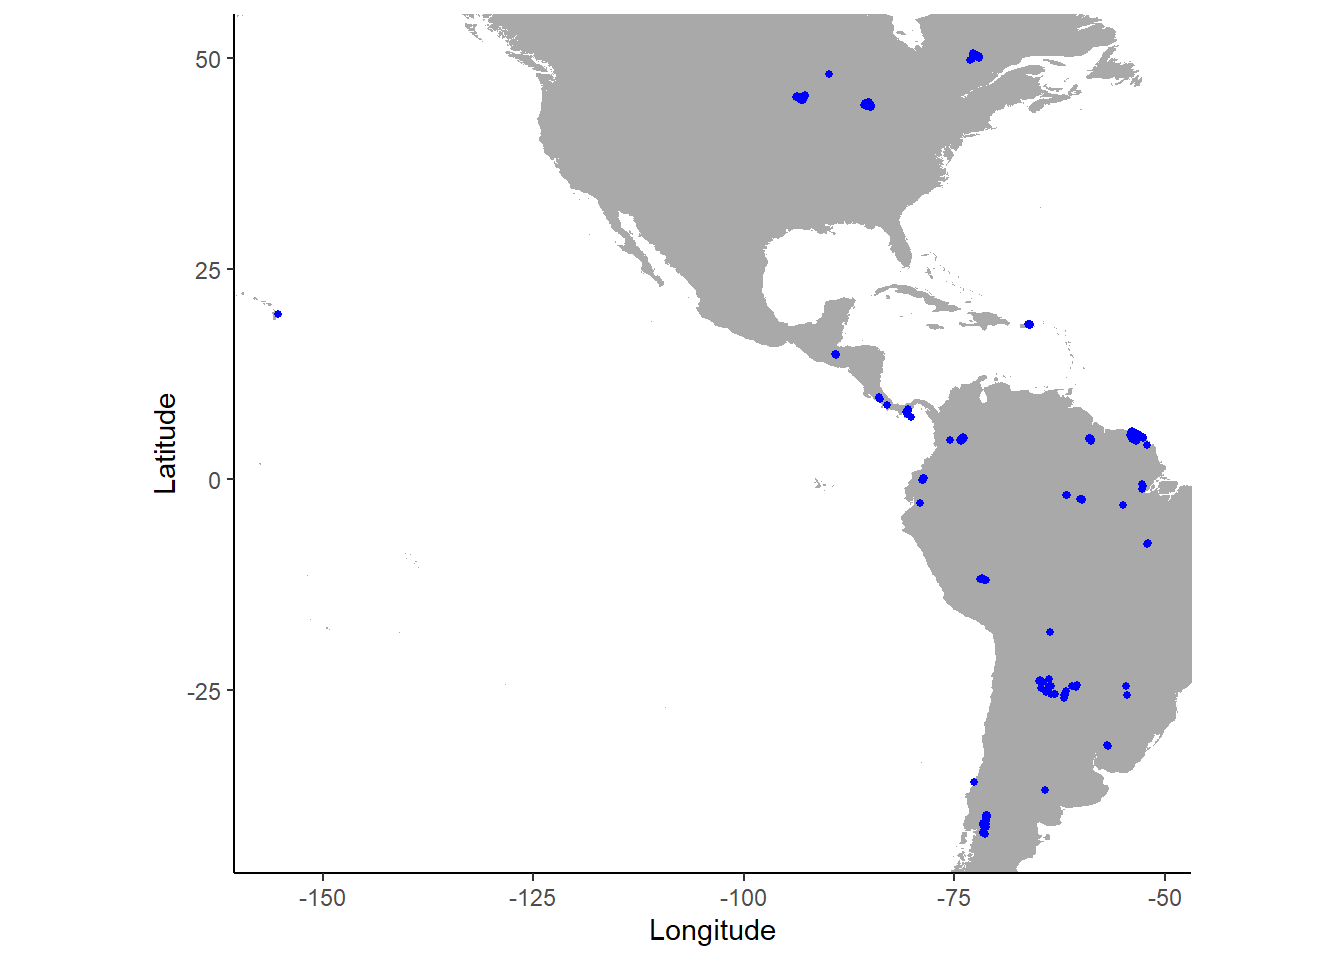
\includegraphics{Practise_Functional_Intactness_Index_files/figure-latex/site visulaisation-1.pdf}
Because the PREDICTS database is a collation of different studies that
often differ in the way data is collected, what is recorded and the
sampling effort expended we need to correct for this assuming that the
biodiversity metric recorded increases linearly with effort.
Additionally, for the diversity metrics that we are going to be
calculating records of abundance and occurrence are useful therefore
studies that record the species richness of sites are dropped

\begin{Shaded}
\begin{Highlighting}[]
\NormalTok{PREDICTS\_Aves\_Am }\OtherTok{\textless{}{-}}\NormalTok{ PREDICTS\_Aves\_Am }\SpecialCharTok{\%\textgreater{}\%} 
  
  
\NormalTok{  dplyr}\SpecialCharTok{::}\FunctionTok{group\_by}\NormalTok{(SS) }\SpecialCharTok{\%\textgreater{}\%} \DocumentationTok{\#\# group by study }
  
\NormalTok{  dplyr}\SpecialCharTok{::}\FunctionTok{mutate}\NormalTok{(}\AttributeTok{Max\_Sampling\_Effort =} \FunctionTok{max}\NormalTok{(Sampling\_effort)) }\SpecialCharTok{\%\textgreater{}\%}  \CommentTok{\# max samplin effort in each site}
  
\NormalTok{  dplyr}\SpecialCharTok{::}\FunctionTok{ungroup}\NormalTok{() }\SpecialCharTok{\%\textgreater{}\%}
  
\NormalTok{  dplyr}\SpecialCharTok{::}\FunctionTok{mutate}\NormalTok{(}\AttributeTok{Rescaled\_Sampling\_Effort =}\NormalTok{ Sampling\_effort}\SpecialCharTok{/}\NormalTok{Max\_Sampling\_Effort) }\SpecialCharTok{\%\textgreater{}\%}  \DocumentationTok{\#\# rescale sampling effort so that the maximum effort with a study is 1}
  
\NormalTok{  dplyr}\SpecialCharTok{::}\FunctionTok{filter}\NormalTok{(Diversity\_metric\_type }\SpecialCharTok{==}\StringTok{"Abundance"} \SpecialCharTok{|}\NormalTok{ Diversity\_metric\_type }\SpecialCharTok{==}  \StringTok{"Occurrence"}\NormalTok{) }\SpecialCharTok{\%\textgreater{}\%}
  
\NormalTok{  dplyr}\SpecialCharTok{::}\FunctionTok{mutate}\NormalTok{(}\AttributeTok{Effort\_Corrected\_Measurement =} \FunctionTok{ifelse}\NormalTok{(Diversity\_metric\_is\_effort\_sensitive }\SpecialCharTok{==} \ConstantTok{TRUE}\NormalTok{,}
\NormalTok{                                                      Measurement}\SpecialCharTok{/}\NormalTok{Rescaled\_Sampling\_Effort,}
\NormalTok{                                                      Measurement)) }\SpecialCharTok{\%\textgreater{}\%}
  
  \FunctionTok{droplevels}\NormalTok{()}

  \DocumentationTok{\#\# Now the Biodiversity data is ready to be used }
  
  \FunctionTok{write\_rds}\NormalTok{(PREDICTS\_Aves\_Am, }\StringTok{"Functional\_Intactness\_Index/PREDICTS\_Americas\_Aves.rds"}\NormalTok{)}
\end{Highlighting}
\end{Shaded}

\#1.2 Preparing the data: Traits (GBD)

In addition to biodiversity data to calculate measures of functional
diversity information on species functional traits is required.
Functional traits are what determines a species functional role in an
ecosystem and are informative on the species niche. Functional traits
can take a variety of forms such as quantitative traits such as body
size, wing length, migratory distance, or qualitative such as foraging
strategy, reproductive strategy etc.

In this analysis I will be using measurements of 8 morphometric traits
in birds including beak dimensions, wing shape, and tarsus and tail
length. To reduce dimensionality, produce major axes of variation and
account for the positive association between all traits and body size I
will be performing a two-step PCA approach proposed by
\href{https://www.journals.uchicago.edu/doi/full/10.1086/678233}{Trisos
et al.~2014}. To derive independent axes of variation I first
partitioned the traits into those related to locomotion (Tarsus, tail,
wing) and those related to foraging (beak dimensions) and perform a PCA
on each. The first principal component of each will represent the
difference in body size and a further PCA on these two axes will produce
a single body size axis. The second principal component of each PCA will
also be retained to represent meaningful axes of variation in locomotion
and foraging strategies.

\begin{Shaded}
\begin{Highlighting}[]
\NormalTok{PCA\_Data }\OtherTok{\textless{}{-}} \FunctionTok{data.frame}\NormalTok{(PREDICTS\_Aves\_Am[,}\FunctionTok{c}\NormalTok{(}\StringTok{"Jetz\_Name"}\NormalTok{, }\StringTok{"Bill.TotalCulmen"}\NormalTok{, }\StringTok{"Bill.Nares"}\NormalTok{, }\StringTok{"Bill.Width"}\NormalTok{, }\StringTok{"Bill.Depth"}\NormalTok{, }\StringTok{"Tarsus.Length"}\NormalTok{,    }\StringTok{"Kipp.s.Distance"}\NormalTok{, }\StringTok{"Secondary1"}\NormalTok{, }\StringTok{"Wing.Chord"}\NormalTok{, }\StringTok{"Hand.Wing.Index"}\NormalTok{, }\StringTok{"Tail.Length"}\NormalTok{, }\StringTok{"Mass"}\NormalTok{)])}

\NormalTok{PCA\_Data }\OtherTok{\textless{}{-}} \FunctionTok{distinct}\NormalTok{(PCA\_Data, Jetz\_Name, }\AttributeTok{.keep\_all =} \ConstantTok{TRUE}\NormalTok{)}
 

\DocumentationTok{\#\#\#\# Log transform {-} then standardise and centre for a mean of zero and a standard deviation of 1}

\NormalTok{PCA\_Data }\OtherTok{\textless{}{-}} \FunctionTok{data.frame}\NormalTok{(}\AttributeTok{Jetz\_Name =}\NormalTok{ PCA\_Data[,}\DecValTok{1}\NormalTok{], }\FunctionTok{scale}\NormalTok{(}\FunctionTok{log}\NormalTok{(PCA\_Data[}\FunctionTok{c}\NormalTok{(}\DecValTok{2}\SpecialCharTok{:}\DecValTok{12}\NormalTok{)]}\SpecialCharTok{+}\DecValTok{1}\NormalTok{)))}

\DocumentationTok{\#\#\# Perform a PCA on all the traits {-} This is just used to compare the utility of the Two{-}step PCA as opposed to just a single full PCA}

\NormalTok{Full.pca.data }\OtherTok{\textless{}{-}}\NormalTok{ PCA\_Data[,}\FunctionTok{c}\NormalTok{(}\DecValTok{2}\SpecialCharTok{:}\DecValTok{6}\NormalTok{,}\DecValTok{8}\SpecialCharTok{:}\DecValTok{9}\NormalTok{,}\DecValTok{11}\NormalTok{)]}

\NormalTok{Full.pca }\OtherTok{\textless{}{-}} \FunctionTok{prcomp}\NormalTok{(Full.pca.data, }\AttributeTok{center =} \ConstantTok{TRUE}\NormalTok{, }\AttributeTok{scale. =} \ConstantTok{TRUE}\NormalTok{)}

\FunctionTok{summary}\NormalTok{(Full.pca)}
\end{Highlighting}
\end{Shaded}

\begin{verbatim}
## Importance of components:
##                           PC1    PC2    PC3     PC4     PC5     PC6    PC7
## Standard deviation     2.4093 1.0443 0.6888 0.59266 0.40304 0.25688 0.1812
## Proportion of Variance 0.7256 0.1363 0.0593 0.04391 0.02031 0.00825 0.0041
## Cumulative Proportion  0.7256 0.8619 0.9212 0.96512 0.98543 0.99368 0.9978
##                            PC8
## Standard deviation     0.13325
## Proportion of Variance 0.00222
## Cumulative Proportion  1.00000
\end{verbatim}

\begin{Shaded}
\begin{Highlighting}[]
\NormalTok{Full.pca}
\end{Highlighting}
\end{Shaded}

\begin{verbatim}
## Standard deviations (1, .., p=8):
## [1] 2.4092952 1.0443412 0.6887533 0.5926587 0.4030390 0.2568825 0.1812128
## [8] 0.1332502
## 
## Rotation (n x k) = (8 x 8):
##                         PC1          PC2        PC3         PC4          PC5
## Bill.TotalCulmen -0.3389852  0.491911056 -0.3223036  0.16570032 -0.007328109
## Bill.Nares       -0.3041723  0.633849609 -0.1341759  0.12825482 -0.107993102
## Bill.Width       -0.3671611  0.011448340  0.6252673  0.06434389  0.037955144
## Bill.Depth       -0.3760971  0.007446666  0.5454248  0.08144172 -0.079651883
## Tarsus.Length    -0.3144990 -0.463944481 -0.3175052  0.59592658 -0.292501049
## Secondary1       -0.3826485 -0.326828921 -0.1064241  0.06290052  0.149682345
## Wing.Chord       -0.3794099 -0.122069335 -0.2227963 -0.28292959  0.749960937
## Tail.Length      -0.3564135 -0.138235747 -0.1670212 -0.71146827 -0.556862370
##                           PC6         PC7         PC8
## Bill.TotalCulmen  0.141654017  0.07275220  0.69739798
## Bill.Nares       -0.089187637  0.01400299 -0.67189911
## Bill.Width        0.668625442 -0.14264206 -0.03339195
## Bill.Depth       -0.714881129 -0.02064379  0.19117776
## Tarsus.Length     0.008203047 -0.37133705 -0.07995325
## Secondary1        0.052274628  0.83247034 -0.11548209
## Wing.Chord       -0.095136440 -0.36780012 -0.06848756
## Tail.Length       0.044875669 -0.08696616  0.01022260
\end{verbatim}

\begin{Shaded}
\begin{Highlighting}[]
\DocumentationTok{\#\#\# PCA on the Foraging traits {-} Beak Dimensions}

\NormalTok{For.pca.data }\OtherTok{\textless{}{-}}\NormalTok{ PCA\_Data[,}\FunctionTok{c}\NormalTok{(}\DecValTok{2}\SpecialCharTok{:}\DecValTok{5}\NormalTok{)]}

\NormalTok{For.pca }\OtherTok{\textless{}{-}} \FunctionTok{prcomp}\NormalTok{(For.pca.data, }\AttributeTok{center =} \ConstantTok{TRUE}\NormalTok{, }\AttributeTok{scale. =} \ConstantTok{TRUE}\NormalTok{)}
\NormalTok{For.pca}
\end{Highlighting}
\end{Shaded}

\begin{verbatim}
## Standard deviations (1, .., p=4):
## [1] 1.7959753 0.8162798 0.2583252 0.2035394
## 
## Rotation (n x k) = (4 x 4):
##                         PC1        PC2         PC3         PC4
## Bill.TotalCulmen -0.5060151 -0.4782999  0.11310828 -0.70879082
## Bill.Nares       -0.4987003 -0.5162231 -0.07871416  0.69182065
## Bill.Width       -0.4940016  0.5209410  0.68724418  0.11080740
## Bill.Depth       -0.5012076  0.4830770 -0.71323632 -0.08198468
\end{verbatim}

\begin{Shaded}
\begin{Highlighting}[]
\FunctionTok{summary}\NormalTok{(For.pca)}
\end{Highlighting}
\end{Shaded}

\begin{verbatim}
## Importance of components:
##                           PC1    PC2     PC3     PC4
## Standard deviation     1.7960 0.8163 0.25833 0.20354
## Proportion of Variance 0.8064 0.1666 0.01668 0.01036
## Cumulative Proportion  0.8064 0.9730 0.98964 1.00000
\end{verbatim}

\begin{Shaded}
\begin{Highlighting}[]
\DocumentationTok{\#\#\# PCA on the Locomotory traits {-} Tarsus, tail and wing dimensions}

\NormalTok{Loco.pca.data }\OtherTok{\textless{}{-}}\NormalTok{ PCA\_Data[,}\FunctionTok{c}\NormalTok{(}\DecValTok{6}\NormalTok{,}\DecValTok{8}\NormalTok{,}\DecValTok{9}\NormalTok{,}\DecValTok{11}\NormalTok{)]}

\NormalTok{Loco.pca }\OtherTok{\textless{}{-}} \FunctionTok{prcomp}\NormalTok{(Loco.pca.data, }\AttributeTok{center =} \ConstantTok{TRUE}\NormalTok{, }\AttributeTok{scale. =} \ConstantTok{TRUE}\NormalTok{)}
\NormalTok{Loco.pca}
\end{Highlighting}
\end{Shaded}

\begin{verbatim}
## Standard deviations (1, .., p=4):
## [1] 1.8376531 0.6406445 0.4122160 0.2066007
## 
## Rotation (n x k) = (4 x 4):
##                     PC1        PC2        PC3        PC4
## Tarsus.Length 0.4727143 -0.7455852  0.2478215 -0.3990344
## Secondary1    0.5329918 -0.1464122 -0.1323444  0.8227808
## Wing.Chord    0.5082494  0.2958254 -0.7082793 -0.3905257
## Tail.Length   0.4838838  0.5789245  0.6476186 -0.1062686
\end{verbatim}

\begin{Shaded}
\begin{Highlighting}[]
\FunctionTok{summary}\NormalTok{(Loco.pca)}
\end{Highlighting}
\end{Shaded}

\begin{verbatim}
## Importance of components:
##                           PC1    PC2     PC3     PC4
## Standard deviation     1.8377 0.6406 0.41222 0.20660
## Proportion of Variance 0.8442 0.1026 0.04248 0.01067
## Cumulative Proportion  0.8442 0.9468 0.98933 1.00000
\end{verbatim}

\begin{Shaded}
\begin{Highlighting}[]
\DocumentationTok{\#\#\#\# Final PCA on the first Principal component of each of the first PCAs to derive an axis of body size }

\NormalTok{Body.pca.data }\OtherTok{\textless{}{-}} \FunctionTok{data.frame}\NormalTok{(}\AttributeTok{LocoPC1 =}\NormalTok{ Loco.pca}\SpecialCharTok{$}\NormalTok{x[,}\DecValTok{1}\NormalTok{], }\AttributeTok{ForPC1 =}\NormalTok{ For.pca}\SpecialCharTok{$}\NormalTok{x[,}\DecValTok{1}\NormalTok{])}
\NormalTok{Body.pca }\OtherTok{\textless{}{-}} \FunctionTok{prcomp}\NormalTok{(Body.pca.data, }\AttributeTok{center =} \ConstantTok{TRUE}\NormalTok{, }\AttributeTok{scale. =} \ConstantTok{TRUE}\NormalTok{)}

\NormalTok{Body.pca}
\end{Highlighting}
\end{Shaded}

\begin{verbatim}
## Standard deviations (1, .., p=2):
## [1] 1.3233861 0.4986475
## 
## Rotation (n x k) = (2 x 2):
##                PC1       PC2
## LocoPC1  0.7071068 0.7071068
## ForPC1  -0.7071068 0.7071068
\end{verbatim}

\begin{Shaded}
\begin{Highlighting}[]
\FunctionTok{summary}\NormalTok{(Body.pca)}
\end{Highlighting}
\end{Shaded}

\begin{verbatim}
## Importance of components:
##                           PC1    PC2
## Standard deviation     1.3234 0.4986
## Proportion of Variance 0.8757 0.1243
## Cumulative Proportion  0.8757 1.0000
\end{verbatim}

\begin{Shaded}
\begin{Highlighting}[]
\DocumentationTok{\#\#\# Match the independent axes of trait variation to species in PREDICTS }

\NormalTok{PC\_Scores }\OtherTok{\textless{}{-}} \FunctionTok{data.frame}\NormalTok{(}\AttributeTok{Jetz\_Name =}\NormalTok{ PCA\_Data[,}\DecValTok{1}\NormalTok{], }\AttributeTok{Foraging.PCA =}\NormalTok{ For.pca}\SpecialCharTok{$}\NormalTok{x[,}\DecValTok{2}\NormalTok{], }\AttributeTok{Loco.PCA =}\NormalTok{ Loco.pca}\SpecialCharTok{$}\NormalTok{x[,}\DecValTok{2}\NormalTok{], }\AttributeTok{Body.PCA =}\NormalTok{ Body.pca}\SpecialCharTok{$}\NormalTok{x[,}\DecValTok{1}\NormalTok{])}


\DocumentationTok{\#\#\# standardize the PC scores so that the maximum value is 1}

\ControlFlowTok{for}\NormalTok{(col }\ControlFlowTok{in} \FunctionTok{colnames}\NormalTok{(PC\_Scores[,}\SpecialCharTok{{-}}\DecValTok{1}\NormalTok{]))\{}
\NormalTok{  PC\_Scores[,col] }\OtherTok{\textless{}{-}}\NormalTok{ PC\_Scores[,col]}\SpecialCharTok{/}\FunctionTok{max}\NormalTok{(PC\_Scores[,col])}
\NormalTok{\}}
\end{Highlighting}
\end{Shaded}

\#2.1 Calculation of functional metrics: Functional Diversity (Rao's
Quadratic Entropy)

The measure of functional diversity I am going to be using is Rao's
Quadratic entropy (Rao's Q). Rao's Q is calculated as the sum of
pairwise functional distances between species within a assembalage,
weighted by each species abundance. Rao's Q had been widely used in the
literature and has advantages by being able to account for species
relative abundance, a limitation of a number of other measures of
functional diversity. There are a number of ways to calculate functional
distances between species within a community but I will be considering
two common methods, first, euclidean distances as I am working with
quantitative axes of trait variation and second, gower distance another
commonly used method that has been favoured previously with it;s ability
to work with qualitative as well and quantitative data. I will be
calculating each measure of Rao in the \textbf{FD} and \textbf{SYNCSA}
packages respectively.

\begin{Shaded}
\begin{Highlighting}[]
\DocumentationTok{\#\#\#\#\#\#\#\#\#\#\#\#\#\#\#\#\#\#\#\#\#\#\#\#\#\#\#\#\#\#\#\#\#\#\#\#\#\#\#}
\DocumentationTok{\#\#\#\# Functional Diversity of sites \#\#\#\#}
\DocumentationTok{\#\#\#\#\#\#\#\#\#\#\#\#\#\#\#\#\#\#\#\#\#\#\#\#\#\#\#\#\#\#\#\#\#\#\#\#\#\#\#}

\NormalTok{abundance\_data }\OtherTok{\textless{}{-}}\NormalTok{ PREDICTS\_Aves\_Am }\SpecialCharTok{\%\textgreater{}\%}\NormalTok{ dplyr}\SpecialCharTok{::}\FunctionTok{filter}\NormalTok{(Diversity\_metric }\SpecialCharTok{==} \StringTok{"abundance"}\NormalTok{) }\SpecialCharTok{\%\textgreater{}\%}\NormalTok{ dplyr}\SpecialCharTok{::}\FunctionTok{filter}\NormalTok{(Effort\_Corrected\_Measurement }\SpecialCharTok{!=} \DecValTok{0}\NormalTok{) }\SpecialCharTok{\%\textgreater{}\%}
  
  \DocumentationTok{\#\#\# filter out studies of just a single species }
  
\NormalTok{  dplyr}\SpecialCharTok{::}\FunctionTok{group\_by}\NormalTok{(SS) }\SpecialCharTok{\%\textgreater{}\%}\NormalTok{ dplyr}\SpecialCharTok{::}\FunctionTok{mutate}\NormalTok{(}\AttributeTok{study\_n\_species =} \FunctionTok{n\_distinct}\NormalTok{(Jetz\_Name)) }\SpecialCharTok{\%\textgreater{}\%}\NormalTok{ dplyr}\SpecialCharTok{::}\FunctionTok{filter}\NormalTok{(study\_n\_species }\SpecialCharTok{\textgreater{}} \DecValTok{1}\NormalTok{) }\SpecialCharTok{\%\textgreater{}\%} \FunctionTok{ungroup}\NormalTok{() }\SpecialCharTok{\%\textgreater{}\%}  
  
  \DocumentationTok{\#\#\#\# group by Site and Species get abundance if there are some sites that the same species is recorded multiple times }
\NormalTok{  dplyr}\SpecialCharTok{::}\FunctionTok{group\_by}\NormalTok{(SSBS,Jetz\_Name) }\SpecialCharTok{\%\textgreater{}\%}\NormalTok{ dplyr}\SpecialCharTok{::}\FunctionTok{mutate}\NormalTok{(}\AttributeTok{SpeciesSiteAbundance =} \FunctionTok{sum}\NormalTok{(Effort\_Corrected\_Measurement)) }\SpecialCharTok{\%\textgreater{}\%}
  
  
  \FunctionTok{ungroup}\NormalTok{() }\SpecialCharTok{\%\textgreater{}\%}   \FunctionTok{droplevels}\NormalTok{() }\SpecialCharTok{\%\textgreater{}\%}
  
  \DocumentationTok{\#\#\# group by just site to get Total site abundance}
  \FunctionTok{group\_by}\NormalTok{(SSBS) }\SpecialCharTok{\%\textgreater{}\%}\NormalTok{ dplyr}\SpecialCharTok{::}\FunctionTok{mutate}\NormalTok{(}\AttributeTok{TotalSiteAbundance =} \FunctionTok{sum}\NormalTok{(SpeciesSiteAbundance), }\AttributeTok{site\_species =} \FunctionTok{n\_distinct}\NormalTok{(Jetz\_Name)) }\SpecialCharTok{\%\textgreater{}\%}
  
  \FunctionTok{ungroup}\NormalTok{() }\SpecialCharTok{\%\textgreater{}\%}
  
  \DocumentationTok{\#\#\# relative abundance of each species at each site SpeciesSitelevel abundance/TotalSite abundance}
\NormalTok{  dplyr}\SpecialCharTok{::}\FunctionTok{mutate}\NormalTok{(}\AttributeTok{RelativeAbundance =}\NormalTok{ SpeciesSiteAbundance}\SpecialCharTok{/}\NormalTok{TotalSiteAbundance) }\SpecialCharTok{\%\textgreater{}\%}
  
  \FunctionTok{droplevels}\NormalTok{()}


\DocumentationTok{\#\# save the abundance data that will come in use for the modelling}

\FunctionTok{write\_rds}\NormalTok{(abundance\_data, }\AttributeTok{file =} \StringTok{"Functional\_Intactness\_Index/abundance\_data.rds"}\NormalTok{)}


\DocumentationTok{\#\#\#\#\#\#\#\#\#\#\#\#\#\#\#\#\#\#\#\#\#\#\#\#\#\#\#\#\#\#\#\#\#\#\#\#\#\#\#\#\#\#\#\#\#\#\#\#\#\#\#\#\#}
\DocumentationTok{\#\#\#\# Function to calculate Rao\textquotesingle{}s Q for each site \#\#\#\#}
\DocumentationTok{\#\#\#\#\#\#\#\#\#\#\#\#\#\#\#\#\#\#\#\#\#\#\#\#\#\#\#\#\#\#\#\#\#\#\#\#\#\#\#\#\#\#\#\#\#\#\#\#\#\#\#\#}




\NormalTok{Rao\_Q\_Func }\OtherTok{\textless{}{-}} \ControlFlowTok{function}\NormalTok{(data)\{}

\NormalTok{Species\_abundance }\OtherTok{\textless{}{-}} \FunctionTok{data.frame}\NormalTok{(data) }\SpecialCharTok{\%\textgreater{}\%}\NormalTok{ dplyr}\SpecialCharTok{::}\FunctionTok{distinct}\NormalTok{(Jetz\_Name) }\SpecialCharTok{\%\textgreater{}\%} \FunctionTok{droplevels}\NormalTok{()}

\ControlFlowTok{for}\NormalTok{(site }\ControlFlowTok{in} \FunctionTok{levels}\NormalTok{(data}\SpecialCharTok{$}\NormalTok{SSBS))\{}

\NormalTok{  Spp\_abd }\OtherTok{\textless{}{-}}\NormalTok{ data }\SpecialCharTok{\%\textgreater{}\%} \FunctionTok{filter}\NormalTok{(SSBS }\SpecialCharTok{==}\NormalTok{ site) }\SpecialCharTok{\%\textgreater{}\%} \FunctionTok{droplevels}\NormalTok{() }\SpecialCharTok{\%\textgreater{}\%} \FunctionTok{data.frame}\NormalTok{()}

  \ControlFlowTok{if}\NormalTok{(}\FunctionTok{any}\NormalTok{(}\FunctionTok{duplicated}\NormalTok{(Spp\_abd}\SpecialCharTok{$}\NormalTok{Jetz\_Name)))\{}
\NormalTok{    Spp\_abd }\OtherTok{\textless{}{-}}\NormalTok{ Spp\_abd[}\SpecialCharTok{{-}}\FunctionTok{which}\NormalTok{(}\FunctionTok{duplicated}\NormalTok{(Spp\_abd}\SpecialCharTok{$}\NormalTok{Jetz\_Name)),]}
\NormalTok{  \}}

\NormalTok{  Species\_abundance }\OtherTok{\textless{}{-}}\NormalTok{ Species\_abundance }\SpecialCharTok{\%\textgreater{}\%} \FunctionTok{left\_join}\NormalTok{(Spp\_abd[,}\FunctionTok{c}\NormalTok{(}\StringTok{"Jetz\_Name"}\NormalTok{, }\StringTok{"RelativeAbundance"}\NormalTok{)], }\AttributeTok{by =} \StringTok{"Jetz\_Name"}\NormalTok{)}
  \FunctionTok{colnames}\NormalTok{(Species\_abundance)[}\FunctionTok{which}\NormalTok{(}\FunctionTok{colnames}\NormalTok{(Species\_abundance) }\SpecialCharTok{==} \StringTok{"RelativeAbundance"}\NormalTok{)] }\OtherTok{\textless{}{-}} \FunctionTok{paste}\NormalTok{(site)}
\NormalTok{\}}

\FunctionTok{rownames}\NormalTok{(Species\_abundance) }\OtherTok{\textless{}{-}}\NormalTok{ Species\_abundance}\SpecialCharTok{$}\NormalTok{Jetz\_Name}
\NormalTok{Species\_abundance }\OtherTok{\textless{}{-}} \FunctionTok{as.matrix}\NormalTok{(Species\_abundance[,}\SpecialCharTok{{-}}\DecValTok{1}\NormalTok{])}
\NormalTok{Species\_abundance[}\FunctionTok{is.na}\NormalTok{(Species\_abundance)] }\OtherTok{\textless{}{-}} \DecValTok{0}  
      


\NormalTok{traits }\OtherTok{\textless{}{-}} \FunctionTok{data.frame}\NormalTok{(data) }\SpecialCharTok{\%\textgreater{}\%}\NormalTok{ dplyr}\SpecialCharTok{::}\FunctionTok{distinct}\NormalTok{(Jetz\_Name) }\SpecialCharTok{\%\textgreater{}\%} \FunctionTok{droplevels}\NormalTok{() }\SpecialCharTok{\%\textgreater{}\%} \FunctionTok{left\_join}\NormalTok{(PC\_Scores, }\AttributeTok{by =} \StringTok{"Jetz\_Name"}\NormalTok{)}
\FunctionTok{rownames}\NormalTok{(traits) }\OtherTok{\textless{}{-}}\NormalTok{ traits}\SpecialCharTok{$}\NormalTok{Jetz\_Name}
\NormalTok{traits }\OtherTok{\textless{}{-}}\NormalTok{ traits[,}\SpecialCharTok{{-}}\DecValTok{1}\NormalTok{]}



\NormalTok{Rao\_Gow }\OtherTok{\textless{}{-}} \FunctionTok{rao.diversity}\NormalTok{(}\AttributeTok{comm =} \FunctionTok{t}\NormalTok{(Species\_abundance),}\AttributeTok{traits =}\NormalTok{  traits)    }\CommentTok{\#THIS is using the package SYNCSA that calcuates Rao\textquotesingle{}s using gowdis dbFD uses euclidean distances}
\CommentTok{\# which i think is better as al the PCs are quantitative and gowdis is useful when there are some qualitative traits as well.}

\NormalTok{Rao\_Euc }\OtherTok{\textless{}{-}}\NormalTok{ FD}\SpecialCharTok{::}\FunctionTok{dbFD}\NormalTok{(}\AttributeTok{x =}\NormalTok{ traits, }\AttributeTok{a =} \FunctionTok{t}\NormalTok{(Species\_abundance))}
\NormalTok{Rao }\OtherTok{\textless{}{-}} \FunctionTok{data.frame}\NormalTok{(}\AttributeTok{Euc =} \FunctionTok{as.numeric}\NormalTok{(Rao\_Euc}\SpecialCharTok{$}\NormalTok{RaoQ), }\AttributeTok{Gow =}\NormalTok{ Rao\_Gow}\SpecialCharTok{$}\NormalTok{FunRao)}



\FunctionTok{return}\NormalTok{(Rao)}
\NormalTok{\}}



\NormalTok{PREDICTS\_Site\_Rao }\OtherTok{\textless{}{-}} \FunctionTok{data.frame}\NormalTok{(abundance\_data) }\SpecialCharTok{\%\textgreater{}\%} \FunctionTok{distinct}\NormalTok{(SSBS, }\AttributeTok{.keep\_all =} \ConstantTok{TRUE}\NormalTok{)}\SpecialCharTok{\%\textgreater{}\%}\NormalTok{ dplyr}\SpecialCharTok{::}\FunctionTok{select}\NormalTok{(SSBS,LandUse, Use\_intensity, LandUse\_Intensity, Longitude,Latitude, site\_species)}

\NormalTok{PREDICTS\_Site\_Rao}\SpecialCharTok{$}\NormalTok{SSBS }\OtherTok{\textless{}{-}} \FunctionTok{as.character}\NormalTok{(PREDICTS\_Site\_Rao}\SpecialCharTok{$}\NormalTok{SSBS)}
\NormalTok{PREDICTS\_Site\_Rao}\SpecialCharTok{$}\NormalTok{Gow\_Rao }\OtherTok{\textless{}{-}} \ConstantTok{NA}
\NormalTok{PREDICTS\_Site\_Rao}\SpecialCharTok{$}\NormalTok{Euc\_Rao }\OtherTok{\textless{}{-}} \ConstantTok{NA}


\NormalTok{Rao\_data }\OtherTok{\textless{}{-}} \FunctionTok{Rao\_Q\_Func}\NormalTok{(abundance\_data)}

\NormalTok{PREDICTS\_Site\_Rao}\SpecialCharTok{$}\NormalTok{Gow\_Rao }\OtherTok{\textless{}{-}}\NormalTok{ Rao\_data}\SpecialCharTok{$}\NormalTok{Gow}
\NormalTok{PREDICTS\_Site\_Rao}\SpecialCharTok{$}\NormalTok{Euc\_Rao }\OtherTok{\textless{}{-}}\NormalTok{ Rao\_data}\SpecialCharTok{$}\NormalTok{Euc}

\FunctionTok{hist}\NormalTok{(PREDICTS\_Site\_Rao}\SpecialCharTok{$}\NormalTok{Gow\_Rao)}
\end{Highlighting}
\end{Shaded}

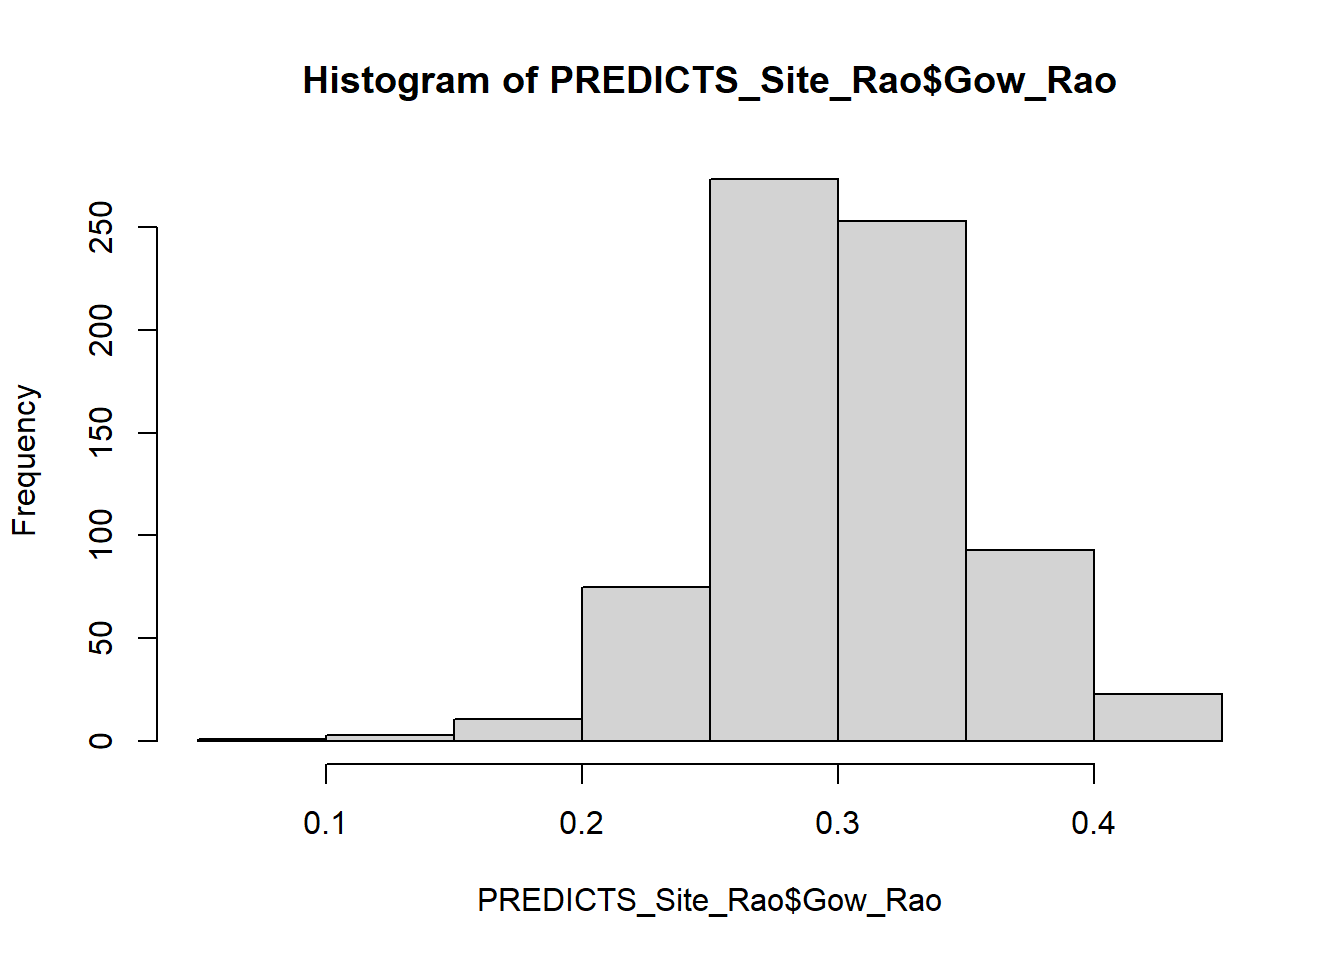
\includegraphics{Practise_Functional_Intactness_Index_files/figure-latex/Raos-1.pdf}

\begin{Shaded}
\begin{Highlighting}[]
\FunctionTok{hist}\NormalTok{(PREDICTS\_Site\_Rao}\SpecialCharTok{$}\NormalTok{Euc\_Rao)}
\end{Highlighting}
\end{Shaded}

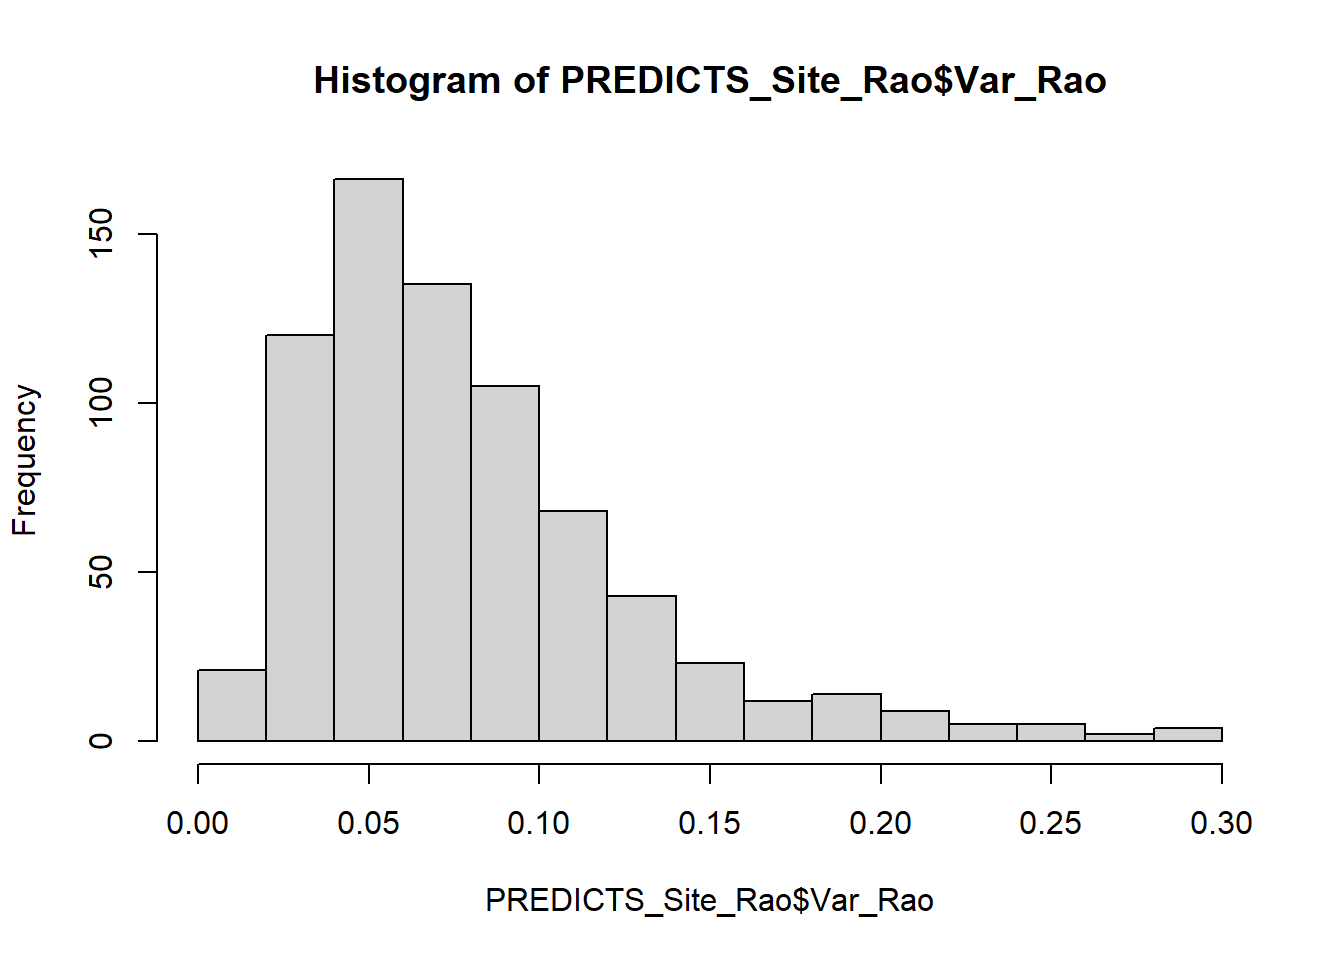
\includegraphics{Practise_Functional_Intactness_Index_files/figure-latex/Raos-2.pdf}

\begin{Shaded}
\begin{Highlighting}[]
\FunctionTok{plot}\NormalTok{(PREDICTS\_Site\_Rao}\SpecialCharTok{$}\NormalTok{Gow\_Rao }\SpecialCharTok{\textasciitilde{}}\NormalTok{ PREDICTS\_Site\_Rao}\SpecialCharTok{$}\NormalTok{Euc\_Rao)}
\end{Highlighting}
\end{Shaded}

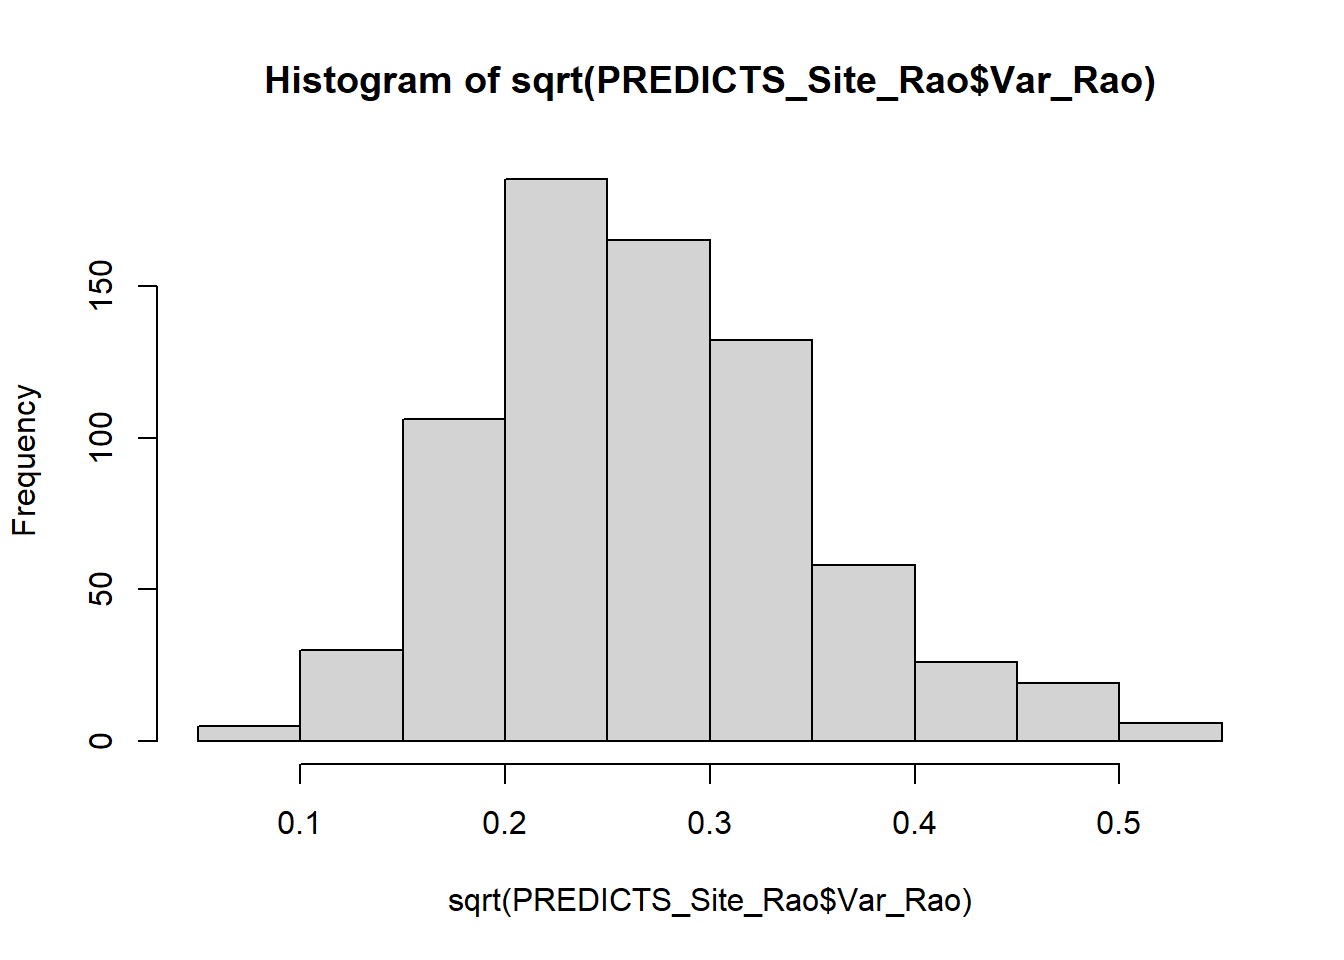
\includegraphics{Practise_Functional_Intactness_Index_files/figure-latex/Raos-3.pdf}

\begin{Shaded}
\begin{Highlighting}[]
\FunctionTok{write\_rds}\NormalTok{(PREDICTS\_Site\_Rao, }\AttributeTok{file =} \StringTok{"Functional\_Intactness\_Index/PREDICTS\_Site\_Rao.rds"}\NormalTok{)}
\end{Highlighting}
\end{Shaded}

\#2.2 Calculation of functional metric: Function similarity

Our second metric I am going to calculate it functional similarity which
is measured as the overlap of hypervolumes in multidimensional trait
space. Essentially we want to know how much functional overlap there is
between Primary minimal sites and sites of other land-use types and
intensities. As previously mentioned the overlap of hypervolumes is not
a full measure of beta-diversity as it only considers the function that
is retain between the two sites and not the changes that occur beyond
those bounds which may be substantial. Some additional analyses would
look more closely at the change in functional structure as a result of
environmental change by partitioning beta-diversity into nestedness
(differences due to shrinking of function) and turnover( differences due
to replacement), with each with different conservation requirements, but
I digress.

Hypervolumes in multidimensional space are defined by the species that
occur at each site that their associated trait scores, here in three
dimensions relating to the PC axes of body, foraging and locomotion
traits. I will construct the hypervolumes using the \textbf{hypervolume}
package developed by B. Blonder, and in two different ways. First I will
create a minimum convex hull that incorporates all points, however this
has some downfalls as it assumes that all space between points is
occupied no matter how disparate they are and can lead to overestimation
of hypervolume size and inaccuracies in overlap calculation. Therefore,
secondly, I will be using a more restrictive decision based algorithm to
construct the hypervolume called a \textbf{One-Class Support Vector
Machine} which randomly generates points in multidimensional trait space
and decides whether it is ``in'' or ``out'' of the boundaries of the
hypervolume with enough samples the points define the hypervolume in
trait space.

To accurately calculate the hypervolumes and their overlap I have only
included sites that have greater that 21 records of species occurrence
or abundance.

\begin{Shaded}
\begin{Highlighting}[]
\DocumentationTok{\#\#\#\#\#\#\#\#\#\#\#\#\#\#\#\#\#\#\#\#\#\#\#\#\#\#\#\#\#\#\#\#\#\#\#\#\#\#\#\#\#\#\#\#\#}
\DocumentationTok{\#\#\#\# Functional Similarity between sites \#\#\#\#}
\DocumentationTok{\#\#\#\#\#\#\#\#\#\#\#\#\#\#\#\#\#\#\#\#\#\#\#\#\#\#\#\#\#\#\#\#\#\#\#\#\#\#\#\#\#\#\#\#\#}


\NormalTok{Similarity\_data }\OtherTok{\textless{}{-}} \FunctionTok{data.frame}\NormalTok{(PREDICTS\_Aves\_Am) }\SpecialCharTok{\%\textgreater{}\%} \FunctionTok{left\_join}\NormalTok{(PC\_Scores, }\AttributeTok{by =} \StringTok{"Jetz\_Name"}\NormalTok{) }\SpecialCharTok{\%\textgreater{}\%} \FunctionTok{filter}\NormalTok{(Effort\_Corrected\_Measurement }\SpecialCharTok{\textgreater{}} \DecValTok{0}\NormalTok{) }\SpecialCharTok{\%\textgreater{}\%}
  
   \DocumentationTok{\#\#\# calculating a hypervolume in 3 dimensions with fewer than 21 species on result in inaccurcies }
  \FunctionTok{group\_by}\NormalTok{(SSBS) }\SpecialCharTok{\%\textgreater{}\%}\NormalTok{ dplyr}\SpecialCharTok{::}\FunctionTok{mutate}\NormalTok{(}\AttributeTok{Site\_spp =} \FunctionTok{n\_distinct}\NormalTok{(Jetz\_Name)) }\SpecialCharTok{\%\textgreater{}\%} \FunctionTok{filter}\NormalTok{(Site\_spp }\SpecialCharTok{\textgreater{}} \DecValTok{21}\NormalTok{) }\SpecialCharTok{\%\textgreater{}\%} \FunctionTok{ungroup}\NormalTok{() }\SpecialCharTok{\%\textgreater{}\%}
  
  \DocumentationTok{\#\# how many studies have at least one site of primary minimal for comparisons to be made and make sure the sites have more than a single site. }
  
  \FunctionTok{group\_by}\NormalTok{(SS) }\SpecialCharTok{\%\textgreater{}\%}\NormalTok{ dplyr}\SpecialCharTok{::}\FunctionTok{mutate}\NormalTok{(}\AttributeTok{n\_primary\_min =} \FunctionTok{sum}\NormalTok{(LandUse\_Intensity }\SpecialCharTok{==} \StringTok{"Primary\_Minimal use"}\NormalTok{ ), }\AttributeTok{n\_sites\_within\_studies =} \FunctionTok{n\_distinct}\NormalTok{(SSBS)) }\SpecialCharTok{\%\textgreater{}\%}
  
  
  \FunctionTok{ungroup}\NormalTok{() }\SpecialCharTok{\%\textgreater{}\%} \FunctionTok{filter}\NormalTok{(n\_primary\_min }\SpecialCharTok{\textgreater{}} \DecValTok{0}\NormalTok{ ) }\SpecialCharTok{\%\textgreater{}\%}  \FunctionTok{filter}\NormalTok{(n\_sites\_within\_studies }\SpecialCharTok{\textgreater{}} \DecValTok{1}\NormalTok{) }\SpecialCharTok{\%\textgreater{}\%}
  
  \FunctionTok{droplevels}\NormalTok{() }\SpecialCharTok{\%\textgreater{}\%}
  
  \FunctionTok{data.frame}\NormalTok{()}

\FunctionTok{write\_rds}\NormalTok{(Similarity\_data, }\AttributeTok{file =} \StringTok{"Functional\_Intactness\_Index/similarity\_data.rds"}\NormalTok{)}




\DocumentationTok{\#\#\#\#\#\#\#\#\#\#\#\#\#\#\#\#\#\#\#\#\#\#\#\#\#\#\#\#\#\#\#\#\#\#\#\#\#\#\#\#\#\#\#\#\#\#\#\#\#\#\#\#\#\#\#\#}
\DocumentationTok{\#\#\#\#\#\# Loop to generate functional overlap of sites \#\#\#\#}
\DocumentationTok{\#\#\#\#\#\#\#\#\#\#\#\#\#\#\#\#\#\#\#\#\#\#\#\#\#\#\#\#\#\#\#\#\#\#\#\#\#\#\#\#\#\#\#\#\#\#\#\#\#\#\#\#\#\#\#\#}

\DocumentationTok{\#\#\# With studies with multiple pri{-}min sites it compares with each other twice {-}{-} prim1 v prim2 \& prim2 v prim 1 etc etc should only really compare once therefore i have create a function that will remove the duplicated comparisons.}

\NormalTok{remove\_dupl\_comparisons }\OtherTok{\textless{}{-}} \ControlFlowTok{function}\NormalTok{(data)\{}

\NormalTok{  data}\SpecialCharTok{$}\NormalTok{drop }\OtherTok{\textless{}{-}} \ConstantTok{NA}
\NormalTok{  data}\SpecialCharTok{$}\NormalTok{comparison }\OtherTok{\textless{}{-}} \FunctionTok{paste}\NormalTok{(data}\SpecialCharTok{$}\NormalTok{site1,data}\SpecialCharTok{$}\NormalTok{site2, }\AttributeTok{sep =} \StringTok{"\_"}\NormalTok{)}
\NormalTok{  data[}\DecValTok{1}\NormalTok{,}\StringTok{"drop"}\NormalTok{] }\OtherTok{\textless{}{-}} \ConstantTok{FALSE}
  
  \ControlFlowTok{if}\NormalTok{(}\FunctionTok{NROW}\NormalTok{(data) }\SpecialCharTok{\textgreater{}} \DecValTok{1}\NormalTok{ )\{}
  
  \ControlFlowTok{for}\NormalTok{(i }\ControlFlowTok{in} \DecValTok{2}\SpecialCharTok{:}\FunctionTok{NROW}\NormalTok{(data))\{}
  
\NormalTok{    site1 }\OtherTok{\textless{}{-}}\NormalTok{ data[i,}\StringTok{"site1"}\NormalTok{]}
\NormalTok{    site2 }\OtherTok{\textless{}{-}}\NormalTok{ data[i,}\StringTok{"site2"}\NormalTok{]}
    
\NormalTok{    match\_1 }\OtherTok{\textless{}{-}} \FunctionTok{as.numeric}\NormalTok{(}\FunctionTok{grep}\NormalTok{(data[}\DecValTok{1}\SpecialCharTok{:}\NormalTok{i}\DecValTok{{-}1}\NormalTok{,}\StringTok{"comparison"}\NormalTok{], }\AttributeTok{pattern =}\NormalTok{ site1))}
\NormalTok{    match\_2 }\OtherTok{\textless{}{-}} \FunctionTok{as.numeric}\NormalTok{(}\FunctionTok{grep}\NormalTok{(data[}\DecValTok{1}\SpecialCharTok{:}\NormalTok{i}\DecValTok{{-}1}\NormalTok{,}\StringTok{"comparison"}\NormalTok{], }\AttributeTok{pattern =}\NormalTok{ site2))}
    
    \ControlFlowTok{if}\NormalTok{(}\FunctionTok{any}\NormalTok{(match\_1 }\SpecialCharTok{\%in\%}\NormalTok{ match\_2))\{}
\NormalTok{      data[i,}\StringTok{"drop"}\NormalTok{] }\OtherTok{\textless{}{-}} \ConstantTok{TRUE}
\NormalTok{    \} }\ControlFlowTok{else}\NormalTok{ \{}
\NormalTok{      data[i,}\StringTok{"drop"}\NormalTok{] }\OtherTok{\textless{}{-}} \ConstantTok{FALSE}
\NormalTok{    \}}
    
\NormalTok{  \}}
    
  \ControlFlowTok{if}\NormalTok{(}\FunctionTok{any}\NormalTok{(data}\SpecialCharTok{$}\NormalTok{drop))\{}
\NormalTok{  data }\OtherTok{\textless{}{-}}\NormalTok{ data[}\SpecialCharTok{{-}}\FunctionTok{which}\NormalTok{(data}\SpecialCharTok{$}\NormalTok{drop }\SpecialCharTok{==} \ConstantTok{TRUE} \SpecialCharTok{\&}\NormalTok{ data}\SpecialCharTok{$}\NormalTok{Contrast }\SpecialCharTok{==} \StringTok{"Primary\_Minimal use{-}Primary\_Minimal use"}\NormalTok{),}\SpecialCharTok{{-}}\FunctionTok{which}\NormalTok{(}\FunctionTok{colnames}\NormalTok{(data) }\SpecialCharTok{==} \StringTok{"comparison"} \SpecialCharTok{|} \FunctionTok{colnames}\NormalTok{(data) }\SpecialCharTok{==} \StringTok{"drop"}\NormalTok{)]}
\NormalTok{  \}}
    
\NormalTok{  \}}
  \FunctionTok{return}\NormalTok{(data)}
\NormalTok{\}}


\DocumentationTok{\#\#\# What studies do we have in the dataset }

\NormalTok{studies }\OtherTok{\textless{}{-}} \FunctionTok{levels}\NormalTok{(Similarity\_data}\SpecialCharTok{$}\NormalTok{SS) }

\DocumentationTok{\#\#\#\# empty data frame for results to go into }





\FunctionTok{registerDoParallel}\NormalTok{(}\AttributeTok{cores =} \DecValTok{4}\NormalTok{)}

\NormalTok{Overlap\_data }\OtherTok{\textless{}{-}} \FunctionTok{foreach}\NormalTok{(}\AttributeTok{study =}\NormalTok{ studies,}
                         \AttributeTok{.combine =} \StringTok{"rbind"}\NormalTok{,}
                         \AttributeTok{.packages =} \FunctionTok{c}\NormalTok{(}\StringTok{"hypervolume"}\NormalTok{,}\StringTok{"betapart"}\NormalTok{,}\StringTok{"tidyverse"}\NormalTok{,}\StringTok{"magrittr"}\NormalTok{,}\StringTok{"geosphere"}\NormalTok{,}\StringTok{"gower"}\NormalTok{,}\StringTok{"raster"}\NormalTok{)) }\SpecialCharTok{\%dopar\%}\NormalTok{ \{}


  \DocumentationTok{\#\#\# data for study }
\NormalTok{Overlap\_data }\OtherTok{\textless{}{-}} \FunctionTok{c}\NormalTok{()}



\NormalTok{  data }\OtherTok{\textless{}{-}}\NormalTok{ Similarity\_data }\SpecialCharTok{\%\textgreater{}\%} \FunctionTok{filter}\NormalTok{(SS }\SpecialCharTok{==}\NormalTok{ study) }\SpecialCharTok{\%\textgreater{}\%} \FunctionTok{droplevels}\NormalTok{()}
  
  \DocumentationTok{\#\#\# coordinates going to be used to calculate distance between sites}
   
\NormalTok{  LatLong }\OtherTok{\textless{}{-}} \FunctionTok{data.frame}\NormalTok{(data) }\SpecialCharTok{\%\textgreater{}\%} \FunctionTok{distinct}\NormalTok{(SSBS,Latitude,Longitude)}
  
  \DocumentationTok{\#\#\# land use and intensity at each site}
  
\NormalTok{  LandUse }\OtherTok{\textless{}{-}} \FunctionTok{data.frame}\NormalTok{(data) }\SpecialCharTok{\%\textgreater{}\%} \FunctionTok{distinct}\NormalTok{(SSBS, LandUse\_Intensity)}

  \DocumentationTok{\#\#\# which sites are of primary minimal landuse type and intensity  }
  
\NormalTok{  Primary\_sites }\OtherTok{\textless{}{-}}\NormalTok{ LandUse }\SpecialCharTok{\%\textgreater{}\%} \FunctionTok{filter}\NormalTok{(LandUse\_Intensity }\SpecialCharTok{==} \StringTok{"Primary\_Minimal use"}\NormalTok{) }\SpecialCharTok{\%\textgreater{}\%} \FunctionTok{pull}\NormalTok{(SSBS) }\SpecialCharTok{\%\textgreater{}\%} \FunctionTok{as.character}\NormalTok{()}
  
  \DocumentationTok{\#\#\#\# all other sites }
  
\NormalTok{  all\_sites }\OtherTok{\textless{}{-}}\NormalTok{ LandUse }\SpecialCharTok{\%\textgreater{}\%} \FunctionTok{pull}\NormalTok{(SSBS) }\SpecialCharTok{\%\textgreater{}\%} \FunctionTok{as.character}\NormalTok{()}

  

  
  \DocumentationTok{\#\#\#\#\#\# get the comparisons with the primary minimal site and all other sites within the study }
  
\NormalTok{  site\_comparisons }\OtherTok{\textless{}{-}} \FunctionTok{expand.grid}\NormalTok{(Primary\_sites, all\_sites) }\SpecialCharTok{\%\textgreater{}\%} 
\NormalTok{    dplyr}\SpecialCharTok{::}\FunctionTok{rename}\NormalTok{(}\AttributeTok{site1 =}\NormalTok{ Var1, }\AttributeTok{site2 =}\NormalTok{ Var2) }\SpecialCharTok{\%\textgreater{}\%}\NormalTok{ dplyr}\SpecialCharTok{::}\FunctionTok{mutate}\NormalTok{(}\AttributeTok{site1 =} \FunctionTok{as.character}\NormalTok{(site1), }\AttributeTok{site2 =} \FunctionTok{as.character}\NormalTok{(site2)) }\SpecialCharTok{\%\textgreater{}\%}
    \FunctionTok{filter}\NormalTok{(site1 }\SpecialCharTok{!=}\NormalTok{ site2) }\SpecialCharTok{\%\textgreater{}\%}
    \FunctionTok{left\_join}\NormalTok{(LatLong, }\AttributeTok{by =} \FunctionTok{c}\NormalTok{(}\StringTok{"site1"} \OtherTok{=} \StringTok{"SSBS"}\NormalTok{)) }\SpecialCharTok{\%\textgreater{}\%}\NormalTok{ dplyr}\SpecialCharTok{::}\FunctionTok{rename}\NormalTok{(}\AttributeTok{site1Lat =}\NormalTok{ Latitude, }\AttributeTok{site1Long =}\NormalTok{ Longitude) }\SpecialCharTok{\%\textgreater{}\%}
    \FunctionTok{left\_join}\NormalTok{(LatLong, }\AttributeTok{by =} \FunctionTok{c}\NormalTok{(}\StringTok{"site2"} \OtherTok{=} \StringTok{"SSBS"}\NormalTok{)) }\SpecialCharTok{\%\textgreater{}\%}\NormalTok{ dplyr}\SpecialCharTok{::}\FunctionTok{rename}\NormalTok{(}\AttributeTok{site2Lat =}\NormalTok{ Latitude, }\AttributeTok{site2Long =}\NormalTok{ Longitude) }\SpecialCharTok{\%\textgreater{}\%}
    \FunctionTok{left\_join}\NormalTok{(LandUse, }\AttributeTok{by =} \FunctionTok{c}\NormalTok{(}\StringTok{"site1"} \OtherTok{=} \StringTok{"SSBS"}\NormalTok{)) }\SpecialCharTok{\%\textgreater{}\%}\NormalTok{ dplyr}\SpecialCharTok{::}\FunctionTok{rename}\NormalTok{(}\AttributeTok{site1LUI =}\NormalTok{ LandUse\_Intensity) }\SpecialCharTok{\%\textgreater{}\%}
    \FunctionTok{left\_join}\NormalTok{(LandUse, }\AttributeTok{by =} \FunctionTok{c}\NormalTok{(}\StringTok{"site2"} \OtherTok{=} \StringTok{"SSBS"}\NormalTok{)) }\SpecialCharTok{\%\textgreater{}\%}\NormalTok{ dplyr}\SpecialCharTok{::}\FunctionTok{rename}\NormalTok{(}\AttributeTok{site2LUI =}\NormalTok{ LandUse\_Intensity) }\SpecialCharTok{\%\textgreater{}\%}
\NormalTok{    dplyr}\SpecialCharTok{::}\FunctionTok{mutate}\NormalTok{(}\AttributeTok{Contrast =} \FunctionTok{paste}\NormalTok{(site1LUI,site2LUI, }\AttributeTok{sep =} \StringTok{"{-}"}\NormalTok{))}
    
  
\NormalTok{  site\_comparisons }\OtherTok{\textless{}{-}} \FunctionTok{remove\_dupl\_comparisons}\NormalTok{(site\_comparisons)}
  
\NormalTok{  site\_one }\OtherTok{\textless{}{-}} \FunctionTok{as.matrix}\NormalTok{(site\_comparisons[,}\FunctionTok{c}\NormalTok{(}\StringTok{"site1Long"}\NormalTok{, }\StringTok{"site1Lat"}\NormalTok{)])}
\NormalTok{  site\_two }\OtherTok{\textless{}{-}} \FunctionTok{as.matrix}\NormalTok{(site\_comparisons[,}\FunctionTok{c}\NormalTok{(}\StringTok{"site2Long"}\NormalTok{, }\StringTok{"site2Lat"}\NormalTok{)])}
  
\NormalTok{  dist }\OtherTok{\textless{}{-}} \FunctionTok{data.frame}\NormalTok{(}\FunctionTok{distHaversine}\NormalTok{(site\_one,site\_two))}
  

  
\NormalTok{  study\_data }\OtherTok{\textless{}{-}}\NormalTok{ site\_comparisons }\SpecialCharTok{\%\textgreater{}\%}\NormalTok{ dplyr}\SpecialCharTok{::}\FunctionTok{select}\NormalTok{(site1,site2, Contrast, site1Long, site1Lat, site2Long,site2Lat)}
\NormalTok{  study\_data }\OtherTok{\textless{}{-}} \FunctionTok{cbind}\NormalTok{(study\_data, }\AttributeTok{distance =}\NormalTok{ dist[,}\DecValTok{1}\NormalTok{])}
\NormalTok{  study\_data}\SpecialCharTok{$}\NormalTok{SS }\OtherTok{\textless{}{-}}\NormalTok{ study}
\NormalTok{  study\_data}\SpecialCharTok{$}\NormalTok{convex\_overlap }\OtherTok{\textless{}{-}} \ConstantTok{NA}
\NormalTok{  study\_data}\SpecialCharTok{$}\NormalTok{hyper\_overlap }\OtherTok{\textless{}{-}} \ConstantTok{NA}
  
    \ControlFlowTok{for}\NormalTok{(i }\ControlFlowTok{in} \DecValTok{1}\SpecialCharTok{:}\FunctionTok{NROW}\NormalTok{(site\_comparisons))\{}
      
      
      \DocumentationTok{\#\#\#\#\# get the species in both sites being compared }
      
\NormalTok{      site1 }\OtherTok{\textless{}{-}}\NormalTok{ site\_comparisons[i,}\StringTok{"site1"}\NormalTok{]}
\NormalTok{      site1\_spp }\OtherTok{\textless{}{-}}\NormalTok{ Similarity\_data }\SpecialCharTok{\%\textgreater{}\%} \FunctionTok{filter}\NormalTok{(SSBS }\SpecialCharTok{==}\NormalTok{ site1) }\SpecialCharTok{\%\textgreater{}\%} \FunctionTok{distinct}\NormalTok{(Jetz\_Name, }\AttributeTok{.keep\_all =} \ConstantTok{FALSE}\NormalTok{)}
      
\NormalTok{      site1\_data }\OtherTok{\textless{}{-}}\NormalTok{ site1\_spp }\SpecialCharTok{\%\textgreater{}\%} \FunctionTok{left\_join}\NormalTok{(PC\_Scores, }\AttributeTok{by =} \StringTok{"Jetz\_Name"}\NormalTok{) }
      \FunctionTok{rownames}\NormalTok{(site1\_data) }\OtherTok{\textless{}{-}}\NormalTok{ site1\_data}\SpecialCharTok{$}\NormalTok{Jetz\_Name}
\NormalTok{      site1\_data }\OtherTok{\textless{}{-}} \FunctionTok{as.matrix}\NormalTok{(site1\_data[,}\SpecialCharTok{{-}}\DecValTok{1}\NormalTok{])}
      
\NormalTok{      hypersvm\_1 }\OtherTok{\textless{}{-}} \FunctionTok{hypervolume}\NormalTok{(site1\_data, }\AttributeTok{method =} \StringTok{"svm"}\NormalTok{)}
\NormalTok{      convex\_1 }\OtherTok{\textless{}{-}} \FunctionTok{expectation\_convex}\NormalTok{(site1\_data, }\AttributeTok{check.memory =} \ConstantTok{FALSE}\NormalTok{)}
      
      
      \DocumentationTok{\#\#\# site 2}
      
\NormalTok{      site2 }\OtherTok{\textless{}{-}}\NormalTok{ site\_comparisons[i,}\StringTok{"site2"}\NormalTok{]}
\NormalTok{      site2\_spp }\OtherTok{\textless{}{-}}\NormalTok{ Similarity\_data }\SpecialCharTok{\%\textgreater{}\%} \FunctionTok{filter}\NormalTok{(SSBS }\SpecialCharTok{==}\NormalTok{ site2) }\SpecialCharTok{\%\textgreater{}\%} \FunctionTok{distinct}\NormalTok{(Jetz\_Name, }\AttributeTok{.keep\_all =} \ConstantTok{FALSE}\NormalTok{)}
      
\NormalTok{      site2\_data }\OtherTok{\textless{}{-}}\NormalTok{ site2\_spp }\SpecialCharTok{\%\textgreater{}\%} \FunctionTok{left\_join}\NormalTok{(PC\_Scores, }\AttributeTok{by =} \StringTok{"Jetz\_Name"}\NormalTok{) }
      \FunctionTok{rownames}\NormalTok{(site2\_data) }\OtherTok{\textless{}{-}}\NormalTok{ site2\_data}\SpecialCharTok{$}\NormalTok{Jetz\_Name}
\NormalTok{      site2\_data }\OtherTok{\textless{}{-}} \FunctionTok{as.matrix}\NormalTok{(site2\_data[,}\SpecialCharTok{{-}}\DecValTok{1}\NormalTok{])}
      
\NormalTok{      hypersvm\_2 }\OtherTok{\textless{}{-}} \FunctionTok{hypervolume}\NormalTok{(site2\_data, }\AttributeTok{method =} \StringTok{"svm"}\NormalTok{)}
\NormalTok{      convex\_2 }\OtherTok{\textless{}{-}} \FunctionTok{expectation\_convex}\NormalTok{(site2\_data, }\AttributeTok{check.memory =} \ConstantTok{FALSE}\NormalTok{)}
      
\NormalTok{      svm\_list }\OtherTok{\textless{}{-}} \FunctionTok{hypervolume\_set}\NormalTok{(hypersvm\_1,hypersvm\_2, }\AttributeTok{check.memory =} \ConstantTok{FALSE}\NormalTok{)}
\NormalTok{      convex\_list }\OtherTok{\textless{}{-}} \FunctionTok{hypervolume\_set}\NormalTok{(convex\_1, convex\_2, }\AttributeTok{check.memory =} \ConstantTok{FALSE}\NormalTok{)}
      
\NormalTok{      svm\_overlap }\OtherTok{\textless{}{-}} \FunctionTok{hypervolume\_overlap\_statistics}\NormalTok{(svm\_list)}
\NormalTok{      convex\_overlap }\OtherTok{\textless{}{-}} \FunctionTok{hypervolume\_overlap\_statistics}\NormalTok{(convex\_list)}
      
\NormalTok{      study\_data[i,}\StringTok{"hyper\_overlap"}\NormalTok{] }\OtherTok{\textless{}{-}}\NormalTok{ svm\_overlap[}\DecValTok{1}\NormalTok{]}
\NormalTok{      study\_data[i,}\StringTok{"convex\_overlap"}\NormalTok{] }\OtherTok{\textless{}{-}}\NormalTok{ convex\_overlap[}\DecValTok{1}\NormalTok{]}

\NormalTok{    \}}

\NormalTok{  Overlap\_data }\OtherTok{\textless{}{-}} \FunctionTok{rbind}\NormalTok{(Overlap\_data,study\_data)}
  

\NormalTok{        \}}


\FunctionTok{write\_rds}\NormalTok{(}\AttributeTok{file =} \StringTok{"Functional\_Intactness\_Index/Functional\_Overlap\_data.rds"}\NormalTok{, Overlap\_data)}


\FunctionTok{registerDoSEQ}\NormalTok{()}
\end{Highlighting}
\end{Shaded}

\#3 Other related pressures

Now that we have the metrics for functional diversity and
similarity/overlap calculated we are almost ready to get on with
modelling how these metrics are impacted by land-use change, however
there are going to be many other pressures that may effect the observed
functional diversity and similarity of a site, therefore we must
consider other factors. Here I calculate the other pressures for each of
the models.

Functional Diversity: Human Population density and density of roads at
1km and 50km radius

Functional Similarity: Human population density, density of road at 1km
and 50 km radius, geographic distance between sites (already calculated
in the previous loop), environmental distance between sites. The
pressure included in the models will be the pressure experienced at
site2 and the difference in pressure between the two sites.

\#\#3.1 Human population density

\begin{Shaded}
\begin{Highlighting}[]
\NormalTok{PREDICTS\_Site\_Rao }\OtherTok{\textless{}{-}} \FunctionTok{readRDS}\NormalTok{(}\StringTok{"Functional\_Intactness\_Index/PREDICTS\_Site\_Rao.rds"}\NormalTok{)}
\NormalTok{Overlap\_data }\OtherTok{\textless{}{-}} \FunctionTok{readRDS}\NormalTok{(}\StringTok{"Functional\_Intactness\_Index/Functional\_Overlap\_data.rds"}\NormalTok{)}



\NormalTok{hpd }\OtherTok{\textless{}{-}} \FunctionTok{raster}\NormalTok{(}\StringTok{"Datasets/PREDICTS\_variables/gpw\_v4\_population\_density\_adjusted\_to\_2015\_unwpp\_country\_totals\_rev11\_2015\_2pt5\_min.tif"}\NormalTok{)}


\DocumentationTok{\#\#\# calculate human population density for Functional diversity sites }

\NormalTok{hpd\_values }\OtherTok{\textless{}{-}}\NormalTok{ raster}\SpecialCharTok{::}\FunctionTok{extract}\NormalTok{(hpd,PREDICTS\_Site\_Rao[,}\FunctionTok{c}\NormalTok{(}\StringTok{"Longitude"}\NormalTok{,}\StringTok{"Latitude"}\NormalTok{)])}

\DocumentationTok{\#\# human population density trandformed with the log +1 transformation}
\NormalTok{PREDICTS\_Site\_Rao}\SpecialCharTok{$}\NormalTok{logHPD }\OtherTok{\textless{}{-}} \FunctionTok{log}\NormalTok{(hpd\_values }\SpecialCharTok{+} \DecValTok{1}\NormalTok{) }



\DocumentationTok{\#\#\# calculate for functional similarity/overlap data}

\NormalTok{hpd\_values\_site1 }\OtherTok{\textless{}{-}}\NormalTok{ raster}\SpecialCharTok{::}\FunctionTok{extract}\NormalTok{(hpd,Overlap\_data[,}\FunctionTok{c}\NormalTok{(}\StringTok{"site1Long"}\NormalTok{,}\StringTok{"site1Lat"}\NormalTok{)])}
\NormalTok{hpd\_values\_site2 }\OtherTok{\textless{}{-}}\NormalTok{ raster}\SpecialCharTok{::}\FunctionTok{extract}\NormalTok{(hpd,Overlap\_data[,}\FunctionTok{c}\NormalTok{(}\StringTok{"site2Long"}\NormalTok{,}\StringTok{"site2Lat"}\NormalTok{)])}

\NormalTok{Overlap\_data}\SpecialCharTok{$}\NormalTok{S1logHPD }\OtherTok{\textless{}{-}} \FunctionTok{log}\NormalTok{(hpd\_values\_site1 }\SpecialCharTok{+} \DecValTok{1}\NormalTok{)}
\NormalTok{Overlap\_data}\SpecialCharTok{$}\NormalTok{S2logHPD }\OtherTok{\textless{}{-}} \FunctionTok{log}\NormalTok{(hpd\_values\_site1 }\SpecialCharTok{+} \DecValTok{1}\NormalTok{)}

\NormalTok{Overlap\_data}\SpecialCharTok{$}\NormalTok{logHPDdiff }\OtherTok{\textless{}{-}}\NormalTok{ Overlap\_data}\SpecialCharTok{$}\NormalTok{S2logHPD }\SpecialCharTok{{-}}\NormalTok{ Overlap\_data}\SpecialCharTok{$}\NormalTok{S1logHPD}
\end{Highlighting}
\end{Shaded}

\#\#3.2 Environmental distance

\begin{Shaded}
\begin{Highlighting}[]
\NormalTok{Bioclim\_5 }\OtherTok{\textless{}{-}} \FunctionTok{raster}\NormalTok{(}\StringTok{"Datasets/Environmental\_Variables/wc2.1\_30s\_bio\_5.tif"}\NormalTok{)}
\NormalTok{Bioclim\_6 }\OtherTok{\textless{}{-}} \FunctionTok{raster}\NormalTok{(}\StringTok{"Datasets/Environmental\_Variables/wc2.1\_30s\_bio\_6.tif"}\NormalTok{)}
\NormalTok{Bioclim\_13 }\OtherTok{\textless{}{-}} \FunctionTok{raster}\NormalTok{(}\StringTok{"Datasets/Environmental\_Variables/wc2.1\_30s\_bio\_13.tif"}\NormalTok{)}
\NormalTok{Bioclim\_14 }\OtherTok{\textless{}{-}} \FunctionTok{raster}\NormalTok{(}\StringTok{"Datasets/Environmental\_Variables/wc2.1\_30s\_bio\_14.tif"}\NormalTok{)}
\NormalTok{Elevation }\OtherTok{\textless{}{-}} \FunctionTok{raster}\NormalTok{(}\StringTok{"Datasets/Environmental\_Variables/wc2.1\_30s\_elev.tif"}\NormalTok{)}


\DocumentationTok{\#\#\# we only have to calculate the environmental distance when comparing two sites.}

\NormalTok{site\_one }\OtherTok{\textless{}{-}} \FunctionTok{as.matrix}\NormalTok{(Overlap\_data[,}\FunctionTok{c}\NormalTok{(}\StringTok{"site1Long"}\NormalTok{,}\StringTok{"site1Lat"}\NormalTok{)])}
\NormalTok{site\_two }\OtherTok{\textless{}{-}} \FunctionTok{as.matrix}\NormalTok{(Overlap\_data[,}\FunctionTok{c}\NormalTok{(}\StringTok{"site2Long"}\NormalTok{,}\StringTok{"site2Lat"}\NormalTok{)])}

\NormalTok{environ\_1 }\OtherTok{\textless{}{-}} \FunctionTok{data.frame}\NormalTok{(}\AttributeTok{Ele  =}\NormalTok{ raster}\SpecialCharTok{::}\FunctionTok{extract}\NormalTok{(Elevation,site\_one), }\AttributeTok{B5 =}\NormalTok{ raster}\SpecialCharTok{::}\FunctionTok{extract}\NormalTok{(Bioclim\_5,site\_one), }\AttributeTok{B6 =}\NormalTok{ raster}\SpecialCharTok{::}\FunctionTok{extract}\NormalTok{(Bioclim\_6, site\_one),}
                        \AttributeTok{B13 =}\NormalTok{ raster}\SpecialCharTok{::}\FunctionTok{extract}\NormalTok{(Bioclim\_13, site\_one), }\AttributeTok{B14 =}\NormalTok{ raster}\SpecialCharTok{::}\FunctionTok{extract}\NormalTok{(Bioclim\_14, site\_one))}

\NormalTok{environ\_2 }\OtherTok{\textless{}{-}} \FunctionTok{data.frame}\NormalTok{(}\AttributeTok{Ele  =}\NormalTok{ raster}\SpecialCharTok{::}\FunctionTok{extract}\NormalTok{(Elevation,site\_two), }\AttributeTok{B5 =}\NormalTok{ raster}\SpecialCharTok{::}\FunctionTok{extract}\NormalTok{(Bioclim\_5,site\_two), }\AttributeTok{B6 =}\NormalTok{ raster}\SpecialCharTok{::}\FunctionTok{extract}\NormalTok{(Bioclim\_6, site\_two),}
                        \AttributeTok{B13 =}\NormalTok{ raster}\SpecialCharTok{::}\FunctionTok{extract}\NormalTok{(Bioclim\_13, site\_two), }\AttributeTok{B14 =}\NormalTok{ raster}\SpecialCharTok{::}\FunctionTok{extract}\NormalTok{(Bioclim\_14, site\_two))}


\NormalTok{environ\_dist }\OtherTok{\textless{}{-}} \FunctionTok{gower\_dist}\NormalTok{(}\AttributeTok{x =}\NormalTok{ environ\_1, }\AttributeTok{y =}\NormalTok{ environ\_2)}
\DocumentationTok{\#\#\#\# I dont know how to best transform it now so Im just going to keep it as is}

\NormalTok{Overlap\_data}\SpecialCharTok{$}\NormalTok{env\_distance }\OtherTok{\textless{}{-}}\NormalTok{ environ\_dist}
\end{Highlighting}
\end{Shaded}

\#\#3.3 Density of Roads

\begin{Shaded}
\begin{Highlighting}[]
\DocumentationTok{\#\#\# load in the roads shape file for the americas}
\NormalTok{Roads }\OtherTok{\textless{}{-}} \FunctionTok{st\_read}\NormalTok{(}\StringTok{"Datasets/PREDICTS\_variables/groads{-}v1{-}americas{-}shp/groads{-}v1{-}americas{-}shp/gROADS{-}v1{-}americas.shp"}\NormalTok{)}
\end{Highlighting}
\end{Shaded}

\begin{verbatim}
## Reading layer `gROADS-v1-americas' from data source `C:\Users\patri\OneDrive - Imperial College London\Work\Biology\(2020-_Natural_History_Museum\PhD_Code\Datasets\PREDICTS_variables\groads-v1-americas-shp\groads-v1-americas-shp\gROADS-v1-americas.shp' using driver `ESRI Shapefile'
## Simple feature collection with 472799 features and 36 fields
## geometry type:  MULTILINESTRING
## dimension:      XY
## bbox:           xmin: -179.9994 ymin: -54.88802 xmax: -32.40191 ymax: 77.22398
## geographic CRS: WGS 84
\end{verbatim}

\begin{Shaded}
\begin{Highlighting}[]
\DocumentationTok{\#\#\# combine into a single shapefile}
\NormalTok{Roads }\OtherTok{\textless{}{-}} \FunctionTok{st\_combine}\NormalTok{(Roads)}
\DocumentationTok{\#\#\# transform to be projected on the mercator projection that deals in meters rather than latlong }
\NormalTok{Roads }\OtherTok{\textless{}{-}} \FunctionTok{st\_transform}\NormalTok{(Roads, }\AttributeTok{crs =} \StringTok{"+proj=merc +ellps=WGS84 +datum=WGS84 +units=m +no\_defs"}\NormalTok{)}

\DocumentationTok{\#\# Both datasets are going to need information on road densities and will be some overlap of sites so make a vector of all unique sites across both datasets}

\NormalTok{sites }\OtherTok{\textless{}{-}} \FunctionTok{unique}\NormalTok{(}\FunctionTok{c}\NormalTok{(Overlap\_data}\SpecialCharTok{$}\NormalTok{site1,Overlap\_data}\SpecialCharTok{$}\NormalTok{site2,PREDICTS\_Site\_Rao}\SpecialCharTok{$}\NormalTok{SSBS))}

\NormalTok{road\_densities }\OtherTok{\textless{}{-}} \FunctionTok{c}\NormalTok{()}

\FunctionTok{registerDoParallel}\NormalTok{(}\AttributeTok{cores =} \DecValTok{4}\NormalTok{)}


\NormalTok{road\_densities }\OtherTok{\textless{}{-}} \FunctionTok{foreach}\NormalTok{(}\AttributeTok{site =}\NormalTok{ sites,}
                          \AttributeTok{.combine =} \StringTok{"rbind"}\NormalTok{,}
                          \AttributeTok{.packages =} \FunctionTok{c}\NormalTok{(}\StringTok{"tidyverse"}\NormalTok{, }\StringTok{"sf"}\NormalTok{, }\StringTok{"rgeos"}\NormalTok{, }\StringTok{"lwgeom"}\NormalTok{)) }\SpecialCharTok{\%dopar\%}\NormalTok{\{}

  
\NormalTok{  site\_LongLat }\OtherTok{\textless{}{-}}\NormalTok{ PREDICTS\_Aves\_Am }\SpecialCharTok{\%\textgreater{}\%} \FunctionTok{filter}\NormalTok{(SSBS }\SpecialCharTok{\%in\%}\NormalTok{ site) }\SpecialCharTok{\%\textgreater{}\%} \FunctionTok{distinct}\NormalTok{(SSBS,Longitude,Latitude)}
  
  
\NormalTok{  point }\OtherTok{\textless{}{-}} \FunctionTok{as.matrix}\NormalTok{(site\_LongLat[,}\FunctionTok{c}\NormalTok{(}\StringTok{"Longitude"}\NormalTok{,}\StringTok{"Latitude"}\NormalTok{)])}
  
\NormalTok{  point }\OtherTok{\textless{}{-}} \FunctionTok{st\_point}\NormalTok{(point)}
\NormalTok{  point }\OtherTok{\textless{}{-}} \FunctionTok{st\_sfc}\NormalTok{(point)}
  
  \FunctionTok{st\_crs}\NormalTok{(point) }\OtherTok{\textless{}{-}} \StringTok{"+proj=longlat +datum=WGS84 +no\_defs"}
\NormalTok{  point }\OtherTok{\textless{}{-}} \FunctionTok{st\_transform}\NormalTok{(point, }\AttributeTok{crs =} \StringTok{"+proj=merc +ellps=WGS84 +datum=WGS84 +units=m +no\_defs"}\NormalTok{)}
  
  
\NormalTok{  buffer\_1km }\OtherTok{\textless{}{-}} \FunctionTok{st\_buffer}\NormalTok{(point, }\DecValTok{1000}\NormalTok{)}
\NormalTok{  buffer\_50km }\OtherTok{\textless{}{-}} \FunctionTok{st\_buffer}\NormalTok{(point, }\DecValTok{50000}\NormalTok{)}
  
  
\NormalTok{  intersect\_1km }\OtherTok{\textless{}{-}} \FunctionTok{st\_intersection}\NormalTok{(Roads, buffer\_1km)}
  
  \ControlFlowTok{if}\NormalTok{(}\FunctionTok{length}\NormalTok{(intersect\_1km) }\SpecialCharTok{!=} \DecValTok{0}\NormalTok{ )\{}
\NormalTok{    density\_1km }\OtherTok{\textless{}{-}}\NormalTok{ (}\FunctionTok{st\_length}\NormalTok{(intersect\_1km)}\SpecialCharTok{/}\DecValTok{1000}\NormalTok{)}\SpecialCharTok{/}\NormalTok{(}\FunctionTok{st\_area}\NormalTok{(buffer\_1km)}\SpecialCharTok{/}\DecValTok{1000000}\NormalTok{)}
\NormalTok{  \} }\ControlFlowTok{else}\NormalTok{ \{}
\NormalTok{    density\_1km }\OtherTok{\textless{}{-}} \DecValTok{0}
\NormalTok{  \}}
  
\NormalTok{  intersect\_50km }\OtherTok{\textless{}{-}} \FunctionTok{st\_intersection}\NormalTok{(Roads, buffer\_50km)}
  
  \ControlFlowTok{if}\NormalTok{(}\FunctionTok{length}\NormalTok{(intersect\_50km) }\SpecialCharTok{!=} \DecValTok{0}\NormalTok{) \{}
\NormalTok{    density\_50km }\OtherTok{\textless{}{-}}\NormalTok{ (}\FunctionTok{st\_length}\NormalTok{(intersect\_50km)}\SpecialCharTok{/}\DecValTok{1000}\NormalTok{)}\SpecialCharTok{/}\NormalTok{(}\FunctionTok{st\_area}\NormalTok{(buffer\_50km)}\SpecialCharTok{/}\DecValTok{1000000}\NormalTok{)}
\NormalTok{  \} }\ControlFlowTok{else}\NormalTok{ \{}
\NormalTok{    density\_50km }\OtherTok{\textless{}{-}} \DecValTok{0}
\NormalTok{  \}}
  
  
\NormalTok{  densities }\OtherTok{\textless{}{-}} \FunctionTok{data.frame}\NormalTok{(}\AttributeTok{site =} \FunctionTok{paste}\NormalTok{(site), }\AttributeTok{density\_1km =} \FunctionTok{as.numeric}\NormalTok{(density\_1km), }\AttributeTok{density\_50km =} \FunctionTok{as.numeric}\NormalTok{(density\_50km))}

\NormalTok{                          \}}

\FunctionTok{registerDoSEQ}\NormalTok{()}


\NormalTok{PREDICTS\_Site\_Rao }\OtherTok{\textless{}{-}}\NormalTok{ PREDICTS\_Site\_Rao }\SpecialCharTok{\%\textgreater{}\%}\NormalTok{ dplyr}\SpecialCharTok{::}\FunctionTok{left\_join}\NormalTok{(road\_densities, }\AttributeTok{by =} \FunctionTok{c}\NormalTok{(}\StringTok{"SSBS"} \OtherTok{=} \StringTok{"site"}\NormalTok{))}

\NormalTok{Overlap\_data }\OtherTok{\textless{}{-}}\NormalTok{ Overlap\_data }\SpecialCharTok{\%\textgreater{}\%}\NormalTok{ dplyr}\SpecialCharTok{::}\FunctionTok{left\_join}\NormalTok{(road\_densities, }\AttributeTok{by =} \FunctionTok{c}\NormalTok{(}\StringTok{"site1"} \OtherTok{=} \StringTok{"site"}\NormalTok{)) }\SpecialCharTok{\%\textgreater{}\%}
\NormalTok{  dplyr}\SpecialCharTok{::}\FunctionTok{rename}\NormalTok{(}\AttributeTok{S1RD1K =}\NormalTok{ density\_1km, }\AttributeTok{S1RD50K =}\NormalTok{ density\_50km) }\SpecialCharTok{\%\textgreater{}\%}
\NormalTok{  dplyr}\SpecialCharTok{::}\FunctionTok{left\_join}\NormalTok{(road\_densities, }\AttributeTok{by =} \FunctionTok{c}\NormalTok{(}\StringTok{"site2"} \OtherTok{=} \StringTok{"site"}\NormalTok{)) }\SpecialCharTok{\%\textgreater{}\%}
\NormalTok{  dplyr}\SpecialCharTok{::}\FunctionTok{rename}\NormalTok{(}\AttributeTok{S2RD1K =}\NormalTok{ density\_1km, }\AttributeTok{S2RD50K =}\NormalTok{ density\_50km)}


\NormalTok{Overlap\_data}\SpecialCharTok{$}\NormalTok{RD1Kdfiff }\OtherTok{\textless{}{-}}\NormalTok{ Overlap\_data}\SpecialCharTok{$}\NormalTok{S2RD1K }\SpecialCharTok{{-}}\NormalTok{ Overlap\_data}\SpecialCharTok{$}\NormalTok{S1RD1K}
\NormalTok{Overlap\_data}\SpecialCharTok{$}\NormalTok{RD50Kdiff }\OtherTok{\textless{}{-}}\NormalTok{ Overlap\_data}\SpecialCharTok{$}\NormalTok{S2RD50K }\SpecialCharTok{{-}}\NormalTok{ Overlap\_data}\SpecialCharTok{$}\NormalTok{S1RD50K}
\end{Highlighting}
\end{Shaded}

\#Save the datasets

\begin{Shaded}
\begin{Highlighting}[]
\FunctionTok{write\_rds}\NormalTok{(}\AttributeTok{file =} \StringTok{"Functional\_Intactness\_Index/Functional\_Overlap\_data.rds"}\NormalTok{, Overlap\_data)}
\FunctionTok{write\_rds}\NormalTok{(}\AttributeTok{file =} \StringTok{"Functional\_Intactness\_Index/PREDICTS\_Site\_Rao.rds"}\NormalTok{, PREDICTS\_Site\_Rao)}
\end{Highlighting}
\end{Shaded}


\end{document}
